\graphicspath{{./figures/hyperblock-scheduling/}}

\chapter{Hyperblock Scheduling}%
\label{sec:hyperblock-scheduling}

\section{Introduction}

% \JW{Something a reader might be curious about: how effective is hyperblock
% scheduling compared to other kinds of scheduling? I mean, is it worth all this
% complexity with hyperblocks? Why not just keep things simple and schedule
% individual basic blocks? Have other people already demonstrated that
% hyperblock-scheduling is significantly better than bb-scheduling? And what
% about its comparison to trace scheduling?}\YH{I think this is answered in the
% second paragraph, although I can move it later.}

High-level synthesis (HLS) is the automatic compilation of
software programs into custom hardware designs. With programmable hardware
devices (such as FPGAs) now widespread, HLS tools such as AMD
Vitis HLS~\cite[]{amd23_vitis_high_synth}, Intel
HLS Compiler~\cite[]{intel20_high_synth_compil},
%Microchip SmartHLS~\cite{smarthls},
LegUp~\cite[]{canis11_legup}, and Bambu~\cite[]{ferrandi21_bambu} are
increasingly relied upon. But existing HLS tools are too unreliable for safety-
and security-critical applications; indeed, random testing by
\textcite{herklotz21_empir_study_reliab_high_level_synth_tools} uncovered
miscompilations in all four of the above tools.

\textcite{herklotz21_formal_verif_high_level_synth} have begun to address this
shortcoming by building \emph{Vericert}, a prototype HLS tool that extends the
CompCert verified C
compiler~\cite{leroy09_formal_verif_compil_back_end}. Vericert guarantees
reliability by being proven correct in Coq, but unfortunately, the hardware
designs it generates cannot compete performance-wise with those generated by
unverified HLS tools. Vericert's key weakness is that it serialises every
operation, taking no advantage of the parallelism that custom hardware offers.

This paper reports on our efforts to close this performance gap by extending
Vericert with a scheduling pass that collects operations into groups that
can be executed in parallel.

\paragraph{Context}
Many approaches to scheduling have been proposed over the years. Some, such as
\emph{list scheduling}~\cite[][p.257]{baker19_princ} only reorder instructions
within a basic block. This means they squander opportunities for performance
improvements that could be obtained by reordering instructions across
branches. A more powerful alternative is \emph{trace
  scheduling}~\cite{ellis85_bulld, fisher81_trace_sched}, which works by
creating paths (or `traces') through the code, across basic-block boundaries,
and then reordering the instructions within those paths. In its most general
form, trace scheduling is considered infeasible on large programs, but two
special cases called \emph{superblock scheduling}~\cite{hwu93_super} and
\emph{hyperblock
  scheduling}~\cite{mahlke92_effec_compil_suppor_predic_execut_using_hyper} have
been developed, both of which impose restrictions on the form of traces in order
to obtain tractable algorithms. Superblocks generalise basic blocks by allowing
early exits, while hyperblocks are basic blocks of \emph{predicated}
instructions. Since hyperblocks are more general than superblocks, and since
predicated execution is easy to implement efficiently in custom hardware,
hyperblock scheduling is a natural fit for HLS. Indeed, the use of hyperblock
scheduling in HLS was first proposed over two decades
ago~\cite{budiu02_compil_applic_specif_hardw,
  callahan98_instr_level_paral_recon_comput}, and is nowadays used by popular
HLS tools such as AMD Vitis HLS~\cite{amd23_vitis_forum},
LegUp~\cite[][p.60]{canis15_legup}, Google XLS~\cite[line~112]{google23_xls},
and Bambu~\cite[line~304]{ferrandi14_panda_bambu}.
% This is due to custom hardware being able to execute arbitrarily many
% independent instructions in parallel.

% \JW{I found a few examples of previous HLS approaches using hyperblock
% scheduling. We could cite them as evidence that hyperblock scheduling is a
% good idea. One example: which is from FPL 2002. Another example: \cite{},
% which is from FPL 1998. Evidence that Vitis uses hyperblock scheduling
% \cite{}}.

\subsubsection*{Contributions}

In this paper, we present:

\begin{itemize}
\item \textbf{the first verified implementation of hyperblock scheduling}, which
  is more general than \citeauthor{six22_formal_verif_super_sched}'s verified
  superblock scheduler~\cite{six22_formal_verif_super_sched} and more
  computationally tractable than
  \citeauthor{tristan08_formal_verif_trans_valid}'s verified trace
  scheduler~\cite{tristan08_formal_verif_trans_valid},
\item \textbf{the first verified implementation of general if-conversion} (a
  pre-scheduling pass that turns if-statements into hyperblocks), building on
  CompCert's na\"ive if-converter that only handles simple
  cases~\cite{absint19_compc},
\item \textbf{a novel use of a verified SAT solver during translation
    validation} in order to reason about predicates, and
\item \textbf{experiments on the widely used PolyBench/C suite} showing that
  scheduling makes Vericert generate 2.1$\times$ faster hardware, thus making it
  competitive with Bambu~\cite{ferrandi21_bambu}, a state-of-the-art
  open-source HLS tool, when a similar set of optimisations is enabled.
\end{itemize}

\section{Overview}
\label{sec:hs:overview}

\Cref{fig:compcert_interm} shows the main components of our hyperblock scheduler
and how they fit into the wider Vericert and CompCert projects.

\definecolor{bgbox1}{HTML}{b3e2cd}
\definecolor{bgbox2}{HTML}{cbd5e8}
\definecolor{bgbox3}{HTML}{fdcdac}
\definecolor{ircolor}{HTML}{e78ac3}

\tikzset{
  numlabel/.style={draw,circle,inner sep=0.5mm,fill=white},
  ir/.style={draw,very thick,black, fill=ircolor!70, align=center},
  pass/.style={draw, very thick, rounded corners, fill=white, align=center},
  extpass/.style={draw, dotted, very thick, rounded corners, fill=white, align=center},
  bgbox/.style={draw=none},
  ed/.style={->, very thick, >=stealth},
}

\begin{figure*}

\centering
\begin{tikzpicture}[
yscale=-1
]
\node[ir] (clight) at (-0.7,0) {\strut Clight};
\node[pass] (ccfront) at (2,0) {CompCert \\ frontend};
\node[ir] (rtl) at (4,0) {\strut \rtl};
\node[pass] (dataflow) at (6,0) {dataflow \\ optimisations};
\node[ir] (ltl) at (8,0) {\strut \ltl};
\node[pass] (ccback) at (10,0) {CompCert \\ backend};
\node[ir] (asm) at (12,0) {\strut asm};

\node[pass] (fsm) at (6,2) {FSM \\ generation};
\node[ir] (htl) at (8,2) {\strut \htl};
\node[pass] (vback) at (10,2) {Vericert \\ backend};
\node[ir] (verilog) at (12,2) {\strut Verilog};

\node[pass] (bbs) at (3.1,2) {\strut find BBs};
\node[ir] (rtlb) at (3.1,4) {\strut \rtlblock};
\node[pass] (ifc) at (0,4) {\strut if-conversion};
\node[pass] (sched) at (5.3,4) {\strut schedule};
\node[ir] (rtlp) at (7.3,4) {\strut \rtlpar};
\node[pass] (fsub) at (10.2,4) {\strut forward  substitution};

\node[anchor=north east, align=right] (cclabel) at (12.8,-1.1)
{CompCert~\cite{leroy09_formal_verif_compil_back_end}};
\begin{pgfonlayer}{background}
\draw[bgbox, fill=bgbox1] (-1.5,-1.1) rectangle (12.8, 0.7);
\end{pgfonlayer}

\node[anchor=north east, align=right] (vlabel) at (12.8,0.9) {Vericert~\cite{herklotz21_formal_verif_high_level_synth}};
\begin{pgfonlayer}{background}
\draw[bgbox, fill=bgbox2] (4.5,0.9) rectangle (12.8, 2.7);
\end{pgfonlayer}

\node[anchor=north east, align=right] (thislabel) at (12.8,2.9) {This work};
\begin{pgfonlayer}{background}
\draw[bgbox, fill=bgbox3] (-1.5,0.9) -- (4.3,0.9) -- (4.3,2.9) -- (12.8,2.9) --(12.8,4.7) -- (-1.5,4.7) -- cycle;
\end{pgfonlayer}

\node[blacknum] at (rtl.north west) {1};
\node[blacknum] at (rtlb.north west) {2};
\node[blacknum] at (bbs.north west) {3};
\node[blacknum] at (ifc.north west) {4};
\node[blacknum] at (rtlp.north west) {5};
\node[blacknum] at (sched.north west) {6};
\node[blacknum] at (fsm.north west) {7};
\node[blacknum] at (fsub.north west) {8};

\draw[ed] (clight) to (ccfront);
\draw[ed] (ccfront) to (rtl);
\draw[ed] (rtl) to (dataflow);
\draw[ed] (dataflow) to (ltl);
\draw[ed] (ltl) to (ccback);
\draw[ed] (ccback) to (asm);
\draw[ed] (rtl) to (fsm);
\draw[ed] (fsm) to (htl);
\draw[ed] (htl) to (vback);
\draw[ed] (vback) to (verilog);
\draw[ed] (rtl) to (bbs);
\draw[ed] (bbs) to (rtlb);
\draw[ed] (rtlb) to[bend left=5] (ifc);
\draw[ed] (ifc) to[bend left=5] (rtlb);
\draw[ed] (rtlb) to (sched);
\draw[ed] (sched) to (rtlp);
\draw[ed] (rtlp) to (fsm);
\draw[ed] (htl) to[bend left=10] (fsub);
\draw[ed] (fsub) to[bend left=10] (htl);

 \end{tikzpicture}
  \caption{New passes and intermediate languages introduced in this work.}%
  \label{fig:compcert_interm}
\end{figure*}

\begin{enumerate}[label=\protect\blacknum{\arabic*}]
\item We intercept the CompCert flow at the Register Transfer
  Language (\rtl).\footnote{Note that this is not the \rtl{} that stands for
    Register-Transfer Level in hardware design.} In \rtl, each function in the
  program is represented as a control-flow graph (CFG) whose nodes are
  individual three-address instructions.
\item We need to identify the basic blocks so they can be combined into
  hyperblocks for scheduling. CompCert has basic-block creation at the Location
  Transfer Language (\ltl), but Vericert's flow has already branched off at
  \rtl. Hence, we define a new intermediate language called \rtlblock, which can
  be thought of as a CFG whose nodes are basic blocks. In order to support
  hyperblocks further along our compilation flow, each instruction is paired
  with a predicate. An instruction is only executed if its predicate evaluates
  to true.
\item We compile from \rtl{} to \rtlblock{} using a \gls{translation validation}
  approach. That is, an unverified algorithm is responsible for gathering
  instructions into basic blocks, then a verified validator confirms the
  equivalence of the \rtl{} and \rtlblock{} representations.  This is similar to
  CompCert's basic-block creation for \ltl{}, but ours is simpler because it is
  not necessary to track variables that may have moved to the stack.
\item We then perform
  if-conversion~\cite{allen83_conver_contr_depen_data_depen}. This is a
  transformation that merges basic blocks from two sides of a fork in the CFG
  into a single, larger basic block (now called a hyperblock) that uses
  predication to control which instructions are executed. If-conversion is
  helpful because larger blocks can give the scheduler more opportunities to
  find parallelism.
  %Our implementation of if-conversion is programmed and
  %verified in Coq.
  CompCert already has an if-conversion pass~\cite{absint19_compc}, but it can
  only handle simple cases such as replacing \texttt{if(p)\{x=a;\}else\{x=b;\}}
  with \texttt{x=p?a:b}, whereas our implementation can handle arbitrary forks
  in the CFG.  If-conversion can be applied selectively, using heuristics to
  judge which basic blocks should be combined. Having proved if-conversion
  correct wherever it is applied, these heuristics can be adjusted with no
  impact on the correctness proof.
%  ======
%Figure XXX: show the four BBs in the CFG for
%
%if(b) { c; } else { d; } e;
%
%then show the one BB in the CFG for
%
%b => c;
%!b => c;
%e;
%======
\item We then perform scheduling on each hyperblock in turn. The scheduler takes
  the list of predicated instructions and produces a list of groups of
  instructions such that all the instructions in the same group can be safely
  executed in parallel. Actually, our scheduler produces a list of groups of
  \emph{lists of} instructions. The idea behind this three-level representation,
  which we call \rtlpar, is that each inner list is a sequence of instructions
  that can be chained together, then each group contains instruction chains that
  can be executed in parallel. In this way, we support \emph{operation
    chaining}, a long-established optimisation in hardware
  design~\cite[p.~1101]{pangrle87_desig_tools_intel_silic_compil}.
\item The scheduler itself is written in unverified OCaml, and works similarly
  to those in existing HLS tools~\cite[]{canis11_legup}: it takes a set of
  scheduling constraints that capture the clock period, available hardware
  resources, and dependencies between operations, encodes them all as a system
  of difference constraints (SDC)~\cite[]{cong06_sdc}, and then hands them off
  to a linear program solver.

\item The CFG is then encoded as a finite state machine (FSM) in a Verilog-like
  language called Hardware Transfer Language (\htl). This process is largely
  inherited from Vericert, but where Vericert produces FSMs that perform just
  one assignment per state, we produce FSM states with a sequence of
  assignments.

\item To ensure that these assignments are actually performed in parallel, we
  have a final pass that performs \emph{forward
    substitution}~\cite[p.~109]{hopwood78_decom} to turn the sequence of Verilog
  blocking assignments into a sequence of non-blocking assignments. For example:
\begin{center}
\begin{tikzpicture}
\node (initial) {\begin{minipage}{0.3\linewidth}
\begin{rtllisting}
a = b * c;
d = a + d;
\end{rtllisting}
\end{minipage}};
\node[right=3cm of initial] (scheduled) {
  \begin{minipage}{0.3\linewidth}
\begin{rtllisting}
a <= b * c;
d <= (b * c) + d;
\end{rtllisting}
  \end{minipage}
};
\draw[-{Latex[length=3mm]}] (initial) -- node [below] {forward substitution}
($(scheduled.west)-(0.5,0)$);
\end{tikzpicture}
\end{center}

The two versions are semantically equivalent, but we find that the second, in
which both right-hand sides must be evaluated before either assignment is
performed, makes the downstream logic synthesis tools more likely to produce the
hardware we intend (which, in this particular example, involves exploiting a
fused multiply--accumulator unit if available).

% ======
% Figure YYY: show how to schedule a little program made up of additions and
% multiplications.
% ======
\end{enumerate}

\noindent
What remains is to ensure the correctness of each schedule produced in step
\blacknum{6}. Following previous work on verified scheduling by
\textcite{tristan08_formal_verif_trans_valid} and
\textcite{six22_formal_verif_super_sched}, we use translation validation, but
dealing with hyperblocks brings additional complexity, as explained below.

\citeauthor{tristan08_formal_verif_trans_valid} implement trace scheduling in
its full generality. They use a tree to represent all the possible control-flow
paths through a block. These trees can be ``exponentially larger than the
original code''~\cite[p.~25]{tristan08_formal_verif_trans_valid}, which makes it
prohibitively expensive to construct and compare the trees before and after
scheduling, and thus undermines the usefulness of their scheduler.

\citeauthor{six22_formal_verif_super_sched} restrict their scheduler to
superblocks. Since a superblock has only a single control-flow path (with early
exits), the need for trees is avoided. This allows their validator to be
``efficient even for large
superblocks''~\cite[p.~53]{six22_formal_verif_super_sched}. However, superblocks
are less general than hyperblocks, and there are code patterns where superblock
scheduling can lead to considerable code duplication that hyperblocks would
avoid. Moreover, superblock scheduling is reliant on profiling and
branch-prediction heuristics to pick a hot path through the program -- should
such a hot path even exist.

Hyperblocks can branch and merge control flow using predicated execution, and
hence a single hyperblock can capture many control-flow paths without the
exponential blow-up that \citeauthor{tristan08_formal_verif_trans_valid}
encountered.  In particular, hyperblocks can handle well the case where two
branches of a conditional statement are executed equally often, unlike the
superblocks that \citeauthor{six22_formal_verif_super_sched} use. However, our
task of validating the equivalence of two hyperblocks is complicated by having
to reason about predicates. Where the prior works only needed to check that the
scheduled block contains a dependency-respecting permutation of the original
block's instructions, we must account for the fact that predicates may be
modified during scheduling. For instance, the sequence %
\rtlinline{p => i; !p => i}, which executes \rtlinline{i} if \rtlinline{p} holds
and then executes \rtlinline{i} if \rtlinline{p} does \emph{not} hold, may be
optimised to \rtlinline{i}.

The approach we take is to translate both the \rtlblock{} hyperblock and the
\rtlpar{} hyperblock (i.e., before and after scheduling) into their strongest
postconditions, starting from the same symbolic initial state, and then
comparing these postconditions for equivalence with the help of a SAT solver
that we have programmed and verified in Coq. By being able to solve queries like
$(\mono{p} \land \mono{!p}) \leftrightarrow \lfalse$, the SAT solver enables
reasoning about reordering of instructions in a predicate-aware fashion.

% This is in contrast to using a tree to represent the control-flow in a block,
% as done by \textcite{tristan08_formal_verif_trans_valid} and in contrast to
% using single traces (paths) through the program as done by
% \textcite{six22_formal_verif_super_sched}.  Specifically, using predicates
% addresses one source of algorithmic complexity that is mentioned by
% \citeauthor*{tristan08_formal_verif_trans_valid}.  Using trees to represent
% control-flow grows exponentially with the number of branches in the
% trace. Instead, by using predicates, common values along different branches in
% the tree are shared, thereby reducing the exponential increase in size and
% checking time.  \JW{This paragraph is v important, but I can't quite follow
% the explanation. Let me try to repeat the argument back to you, to see how
% much I understand. Tristan and Leroy (TL) and Six et al. (S+) both need to
% represent a block before and after scheduling, in order to do the
% validating. TL implement trace scheduling in its full generality. They use a
% tree to represent all the possible control-flow paths through a block, but
% these trees quickly grow very large, so comparing the before-tree and the
% after-tree can take a prohibitively long time, thus undermining the usefulness
% of their scheduler. S+ restrict their scheduling to superblocks, which
% describe a single control-flow path. Thus there's no need for a huge tree of
% possibilities. That solves the complexity problem. Our use of predicates is
% another way to solve that same problem. What I don't get from the explanation
% so far is how our approach compares to S+'s approach. Don't they have some
% weakness to do with relying on unverified hash-consing? And of course there
% are the usual pros and cons of superblock scheduling vs hyperblock scheduling,
% as discussed below. }

%\subsection{Generalising Superblocks to Hyperblocks}

%In contrast to \citeauthor*{six22_formal_verif_super_sched}, we support
% hyperblocks, which offer some additional flexibility when compared to
% superblocks.  In particular, superblocks describe a single path through the
% program, so they do not suffer the same exponential blow-up in equivalence
% checking time.  Because of this, superblock scheduling is reliant on profiling
% and branch-prediction heuristics to pick a hot-path through the
% program. However, cases where there is no single hot-path, such as an
% alternating conditional statement, cannot be represented as a single
% superblock, meaning that these cases cannot be scheduled as a single unit.
% \JW{Is that right? I think they \emph{can} be represented using superblocks,
% but you just have to commit to one branch over the other, which means that the
% scheduler isn't going to do a very good job} \YH{I guess that is what I was
% trying to convey though, that you can't combine two paths in a superblock.
% I'll try to reword it.  Maybe it's a bit clearer with a single superblock}

% Hyperblocks can branching and merging control-flow using predicates, and can
% therefore represent cases where two branches of a conditional statement have
% the same chance of being executed.  In that case, it is beneficial to schedule
% the two conditional branches together to take advantage of any possible
% resource sharing, as well as having more freedom in how instructions can be
% reordered.

% This section describes the structure of hyperblocks in
% \cref{sec:scheduling:hyperblocks}.  Then, the structure of two extra
% intermediate languages that were added to CompCert to implement hyperblocks
% are also shown in \cref{sec:rtlblockdef}.

\section{New Intermediate Languages}%
\label{sec:hs:rtlblockdef}

Our work introduces two new intermediate languages: \rtlblock{} and \rtlpar{},
which implement the sequential and parallel semantics %\YH{I wanted to remove
% parallel semantics everywhere, because we do not actually have parallel
% semantics, so instead I wanted to replace it by ``scheduled hyperblock''.}
of
hyperblocks respectively.  They are based on CompCert's \rtl{}, but instead of
mapping from states to instructions, \rtlblock{} maps from states to
hyperblocks, and \rtlpar{} maps from states to parallel hyperblocks.

%\YH{TODO: Fix control-flow instruction syntax.}
\begin{figure}
\centering
\begin{tabular}{rr@{~}r@{~}l@{\hspace*{2mm}}l}
  \llabel{registers} & $\reg, \mbox{\rtlinline{r1}}, \mbox{\rtlinline{r2}}, \ldots \in \regtype$ & & & \\
  \llabel{predicates} & $\predvar, \mbox{\rtlinline{p1}}, \mbox{\rtlinline{p2}}, \ldots \in \predvartype$ & & & \\
  \llabel{CFG node labels} & $\location \in \locationtype$ & $::=$ & $\mathbb{N}$ & \\
  \llabel{guard expressions} & $\guard \in \guardtype$ & ::= & \rlap{$\predvartype$ | $\neg
                                              \predvartype$ | $\ltrue$ | $\lfalse$ | $\guardtype \land \guardtype$ | $\guardtype \lor \guardtype$} \\
  \llabel{arithmetic ops} & $\exprop \in \exproptype$ & ::= & \mono{+} | \mono{*} | \mono{-} | \ldots & \\
  \llabel{conditional ops} & $\condop \in \condoptype$ & ::= & \mono{==} | \mono{!=} | \mono{<}
                                               | \ldots & \\
  \llabel{addressing modes} & $\addr \in \addrtype$ & ::= & \mono{Stack} | \mono{Global} |
                                             \ldots \\
  \llabel{instructions} & $\instr \in \instrtype$ & ::= & \mono{skip} & \rlabel{no-op}\\
     & & |   & \hl{$\guardtype$ \texttt{\small =>}} $\regtype \casgn \regtype \mathbin{\exproptype} \regtype$ & \rlabel{arith/logical op} \\
     & & |   & \hl{$\guardtype$ \texttt{\small =>}} $\regtype \casgn \at{\addrtype}{\regtype}$ & \rlabel{memory load}\\
     & & |   & \hl{$\guardtype$ \texttt{\small =>}} $\at{\addrtype}{\regtype}$ \mono{:=} $\regtype$ & \rlabel{memory store} \\
     & & |   & \hl{$\guardtype$ \texttt{\small =>} $\predvartype \casgn
               \regtype \mathbin{\condoptype} \regtype$} & \rlabel{assign predicate} \\
     & & |   & \hl{$\guardtype$ \texttt{\small =>} $\mono{E}(\cfinstrtype)$} & \rlabel{block exit}
  \\
  \llabel{control-flow instructions} & $\cfinstr \in \cfinstrtype$ & ::= & \mono{if} $(\regtype \mathbin{\condoptype} \regtype)$ $\locationtype$ $\locationtype$ & \rlabel{conditional} \\
      & & |   & \mono{goto} $\locationtype$ & \rlabel{goto node} \\
      & & |   & \ldots \\
%      & & |   & \mono{call} $\mathit{sig}$ $f$ $\vec{\regtype}$ $\regtype$ $\locationtype$ & (function call)\\
%      & & |   & \mono{tailcall} $\mathit{sig}$ $f$ $\vec{\regtype}$ & (tailcall) \\
%      & & |   & \mono{builtin} $f_{\mathit{ext}}$ $\vec{\regtype}$ $\regtype$ $\locationtype$ & (builtin function) \\
%      & & |   & \mono{jumptable} $\regtype$ $\vec{\locationtype}$ & (jumptable) \\
%      & & |   & \mono{return} $\optiontype{\regtype}$ & (function return) \\
%      % & |   & \mono{RBpred\_{cf}} $P$ $i_{\mathit{cf}_{1}}$
      % $i_{\mathit{cf}_{2}}$ \\
      & \llap{$\rtlbb \in \rtlblock{}$} & ::= & $\instr\ \texttt{list}$ \\
      & \llap{$\rtlpb \in \rtlpar{}$} & ::= & $\instr\ \texttt{list}\ \texttt{list}\ \texttt{list}$
\end{tabular}
\caption{Syntax of \rtlblock{} and \rtlpar{}, with our hyperblock additions \hl{highlighted}.}
\label{fig:instructions}
\end{figure}
% \rtlblock{} instructions are split into two types of instructions, standard
% instructions and control-flow instructions.
Hyperblocks are made up of instructions as defined in \cref{fig:instructions},
where $\vec{\cdot}$ denotes a list and $\optiontype{\cdot}$ denotes an optional
parameter. %$\exprop$ and $\condop$ are standard
% \compcert{} arithmetic and conditional operations, $\reg$ is a register,
% $\addr$ contains address information and the type of memory access being
% performed, $\predvar$ is a
% predicate, %$\mathit{sig}$ is a type signature, $f$ is a function name, $f_{\mathit{ext}}$ is an external function name, and $\location$ denotes the next node in the CFG to jump to.
Most instructions are similar to their \rtl{} counterparts, except each
instruction is now guarded by an optional predicate. One additional instruction
is for setting a predicate ($\predvar$) equal to an evaluated condition
($\reg_1\mathbin{\condop}\reg_2$).
% When this instruction is introduced during if-conversion,
% $\reg_1\mathbin{\condop}\reg_2$ is the if-statement's condition.
The other new instruction is \mono{E}, which takes a control-flow instruction
($\cfinstr$) and allows for early exit from the hyperblock.

% \mono{RBsetpred} is a standard instruction that sets a predicate variable
% ($p$) equal to an evaluated condition ($c$).  This instruction is introduced
% during if-conversion to capture an if-statement's condition in a predicate.
% All other instructions optionally contain a predicate which has been set
% beforehand, which forms the hyperblock.  In addition to that, there is also an
% extra instruction called \mono{RBexit}, which takes an optional predicate and
% a control-flow instruction ($i_{\mathit{cf}}$), and allows for early exit from
% a hyperblock.

These instructions are used in both \rtlblock{} and \rtlpar.  The main
difference between these two languages is how these instructions are arranged
within the hyperblock and the execution semantics of the hyperblock. An
\rtlblock{} hyperblock is a list of instructions, with a straightforward
sequential semantics. An \rtlpar{} hyperblock is list of lists of lists of
instructions, with nested blocks corresponding to where instructions should be
placed in hardware.  Each innermost list contains a chain of instructions that
can be executed sequentially within a single clock cycle; each middle list
contains a group of chains that can be executed in parallel; and the outermost
list contains groups to be executed sequentially (in consecutive clock cycles).

% \JW{Rough notes follow.} The ordinary CompCert semantics for programs $P$ is a mapping from an initial state $\context$ to a final state $\context'$, written:
% \[
% \Gamma \vdash P \Downarrow \Gamma'
% \]
% where $\context$ is a 3-tuple consisting of a `global environment' $\Gamma_{Env}$ that contains global information about the program, a mapping $\forestregset{\context}$ from registers to values, and a mapping $\forestmem{\context}$ from memory addresses to values. In order to handle predicates, in our work we turn $\context$ into a 4-tuple $(\Gamma_{Env}, \forestregset{\context}, \forestpredset{\context}, \forestmem{\context})$, where $\forestpredset{\context}$ maps predicates to Booleans. We also need to be able to give a semantics to individual hyperblocks $B$. For this, we write:
% \[
% \Gamma \vdash B \Downarrow (\Gamma', I)
% \]
% where the additional component $I$ is the instruction in $B$ that is executed to exit the block.

The existing CompCert semantics for \rtl{} is a small-step operational semantics
defined on a CFG. At each step, the instruction in the CFG at the current
program counter is evaluated in a context $\context$. This is a 3-tuple
comprising an environment $\forestenv{\context}$ that has global information
about the program, a mapping $\forestregset{\context}$ from registers to values,
and a mapping $\forestmem{\context}$ from memory addresses to values.

In order to give a semantics for \rtlblock{} and \rtlpar{}, we need to handle
predicates, so we turn $\context$ into a 4-tuple
$(\forestenv{\context}, \forestregset{\context}, \forestpredset{\context},
\forestmem{\context})$, where the additional component
$\forestpredset{\context}$ maps predicates to Booleans.  Moreover, we need to
deal with CFGs where each node is not just a single instruction, but a
hyperblock. The semantics, which we provide in
\cref{fig:semantics-of-rtlblock-and-rtlpar}, is big-step in the sense that it
executes an entire hyperblock in a single step.  The \nameref{rule:execinstr}
rule executes an arithmetic instruction if its guard evaluates to true (and
there are similar rules for the other guarded instructions). The
\nameref{rule:execinstrfalse} rule handles the case where the guard does not
hold. \nameref{rule:execexit} handles the execution of an exit instruction by
recording the control-flow instruction $\cfinstr$ for leaving the block. The
next two rules are for executing an instruction list, with
\nameref{rule:blockcontinue} handling the case where the head instruction does
not exit the block, and \nameref{rule:blockexit} handling the case where it
does. Finally, \nameref{rule:execrtlblock} and \nameref{rule:execrtlpar} provide
the semantics of \rtlblock{} and \rtlpar{} blocks respectively. Both languages
use the list execution semantics defined by the above rules, but \rtlpar{}
blocks are first flattened into a single list (via \mrtl{concat}).

Note that these rules define a sequential semantics for \rtlpar{}. That is,
although \rtlpar{} blocks contain lists of instruction chains that have been
identified by the scheduler as being suitable for parallel execution, our
semantics nonetheless executes them sequentially. This is because although the
scheduler identifies where parallelism can be profitably extracted, the program
does not actually become parallel until the final `forward substitution' pass,
where Verilog blocking assignments become non-blocking assignments. Hence, to
avoid unnecessary complexity, we keep the semantics sequential at the \rtlpar{}
stage. (A parallel \rtlpar{} semantics may allow more optimisations to be
validated, but we save that for future work.)

\newcommand\cons{\mathbin{::}}

\begin{figure}
    \centering
    \begin{mathpar}
        \inferrule[ExecInstr]{\evalop[\forestpredset{\context}]{\guard}{\booleantrue}
          \\ \evalop{\mrtl{r1} \mathbin{\exprop}
            \mrtl{r2}}{v}}{\seminstr{(\guard\ \mrtl{ => rd := r1}
            \mathbin{\exprop} \mrtl{r2})}{((\at{\forestregset{\context}}{\mrtl{rd} \mapsto v},
            \forestpredset{\context}, \forestmem{\context}), \cnone)}}
        \label{rule:execinstr}
        \and
        \inferrule[ExecInstrFalse]{\evalop[\forestpredset{\context}]{\guard}{\booleanfalse}}
        {\seminstr{(\guard\ \mrtl{=>}\ \_)}{(\context, \cnone)}}
        \label{rule:execinstrfalse}
        \and
        \inferrule[ExecExit]{\evalop[\forestpredset{\context}]{\guard}{\booleantrue}}
        {\seminstr{(\guard\ \mrtl{ => E(} \cfinstr \mrtl{)})}{(\context, \some{\cfinstr})}}
        \label{rule:execexit}
        \and
        \inferrule[BlockContinue]{\seminstr{\instr}{(\context',
            \cnone)} \\ \seminstrlist[\context']{l}{(\context'',
            \cfinstr)}}{\seminstrlist[\context]{\instr \cons l}{(\context'', \cfinstr)}}
        \label{rule:blockcontinue}
        \and
        \inferrule[BlockExit]{\seminstr{\instr}{(\context',
            \some{\cfinstr})}}{\seminstrlist{\instr \cons l}{(\context', \cfinstr)}}
        \label{rule:blockexit}
        \and
        \inferrule[ExecRtlBlock]{\seminstrlist{\rtlbb}{(\context',
            \cfinstr)}}{\semrtlblock{\rtlbb}{(\context', \cfinstr)}}
        \label{rule:execrtlblock}
%        \inferrule[RTLBlock]{\at{f}{n} = \some{l} \\ \seminstrlist[]{(l,
%            (\context, \cnone))}{(\context', \some{\cfinstr})} \\
%          \semcfinstr[\environment, \context']{\cfinstr}{(t, \Sigma)}}{\smallsem{\text{\rtlblock}}{}{\mathtt{State}(\mathit{sf}, f, n, \context)}{\Sigma}{t}}
        \and
        \inferrule[ExecRtlPar]{\seminstrlist{\mrtl{concat} (\mrtl{concat}\ \rtlpb)}{(\context',
            \cfinstr)}}{\semrtlpar{\rtlpb}{(\context', \cfinstr)}}
        \label{rule:execrtlpar}
%        \inferrule[RTLPar]{\at{f}{n} = \some{l} \\
%          \seminstrlist[]{(\mathtt{concat}\ (\mathtt{concat}\ l), (\context,
%            \cnone))}{(\context', \some{\cfinstr})} \\ \semcfinstr[\environment,
%          \context']{\cfinstr}{(t, \Sigma)}}{\smallsem{\text{\rtlpar}}{}{\mathtt{State}(\mathit{sf}, f, n, \context)}{\Sigma}{t}}
    \end{mathpar}
    \caption{Semantics of \rtlblock{} and \rtlpar{} hyperblocks. %formulated in
      %terms of the execution of a single instruction
      %$\seminstr[\cdot]{\cdot}{\cdot}$ and a control-flow instruction
      %$\semcfinstr[\cdot]{\cdot}{\cdot}$. %reusing the existing CompCert
      %semantics for most of the operations. Only the rules for the execution of
      % \rtlblock{} and \rtlpar{} from the \texttt{State} state are shown, as the
      % transitions for the \texttt{Call} and \texttt{Return} states are the same
      %as \rtl{}.
      }%
    \label{fig:semantics-of-rtlblock-and-rtlpar}
\end{figure}

% \JW{We should comment, either here or later on, but probably best here, on the
%   fact that you can exit a hyperblock from inside one of those `threads', which
%   is perhaps a bit unintuitive. We considered simplifying things by requiring
%   exits to have nothing in parallel with them, but this leads to wasted clock
%   cycles. }\YH{I think if we make it clear that we do not have parallel
%   semantics then this shouldn't be that confusing anymore.  Instead we can just
%   focus on the fact that the scheduled \rtlpar{} just describes the layout of
%   the instructions, and does not care about them actually being independent.}

%The structure of the basic blocks of these two languages are defined below:
% \begin{center}
% \begin{tabular}{ccl}
%    \blockbb & ::= & $i\ \text{\tt slist}$ \\
%    \parbb   & ::= & $i\ \text{\tt slist}\ \text{\tt plist}\ \text{\tt slist}$\\
%   \end{tabular}
% \end{center}

% \noindent where \blockbb{} defines sequential basic blocks present in
% \rtlblock, and \parbb{} defines the parallel basic blocks present in \rtlpar.
% \JW{This is fine, but I wonder if it's necessary to introduce the \blockbb{}
% and \parbb{} syntax -- you don't use it elsewhere as far as I can see, so it
% only adds to cognitive overhead.}  \Cref{fig:hb_def} shows the different
% nesting levels of the basic blocks in \rtlblock{} as well as \rtlpar.  We see
% that \rtlblock{} is made of a list of instructions, with control-flow
% instructions present anywhere in the block that may exit this block early.
% Each instruction in \rtlblock{} is executed sequentially. \rtlpar{} is made of
% a list of lists of lists.  The outer list behaves like the list in \rtlblock,
% and executes each list inside it sequentially.  \rtlpar{} then has a list that
% executes its contents in parallel, meaning each instruction uses the same
% state of the registers and memory while executing.  Finally, there is an
% additional layer of sequentially executing lists of instructions, to be able
% to execute small groups of instructions in sequence, but still in parallel to
% the other instructions in the current parallel group.

% \rtlpar{} is structured in this way so that the scheduler has more
% flexibility. Instructions can not only be parallelised in the basic blocks,
% but it can also define sequential operations within these parallel operations.
% This is especially useful for the hardware back end, as it means that
% sequential operations that do not quite fill one clock cycle can be executed
% sequentially, but can still be executed in parallel with other independent
% operations.  This optimisation is called operation chaining, and is critical
% to get the most performance out of the hardware.

\section{Verified If-Conversion}%
\label{sec:hs:if-conversion}

If-conversion introduces the predicated instructions that form hyperblocks.  As
mentioned in \cref{sec:overview}, CompCert does have an if-converter already,
but it applies only in a few special cases. We need a more general algorithm
that can handle arbitrary branching code.
% Such code can be represented using non-branching instructions due to the
% predicated instructions introduced in \cref{sec:rtlblockdef}.
We therefore implement the first formally verified implementation of a general
if-conversion algorithm, with support for heuristics for branch prediction.

To simplify both the implementation of the if-converter and its correctness
proof, it is split up into three distinct
transformations:%, as shown in \cref{fig:if-conversion-details}:

% \begin{figure}
%   \centering
%   \begin{tikzpicture}[>=Latex,shorten >=1pt,node distance=1cm and 1cm,%
%     transf/.style={very
%       thick,draw,fill=Orchid!40,font={\sffamily\bfseries},align=center},%
%     exttransf/.style={very
%       thick,draw,fill=Coral!40,font={\sffamily\bfseries},align=center},%
%     conn/.style={very thick,->}]
%     % JW: I switched to the same tikz styles that we used in figure 1, for consistency.
%     \node[pass] (cond elim) {Condition \\ Elimination};
%     \node[pass,below right=of cond elim] (block inlining) {Block \\ Inlining};
%     \node[extpass,right=of block inlining] (external decision) {External \\
%       Decision \\ Procedure};
%     \node[pass,above right=of block inlining] (dead block) {Dead Block \\
%       Elimination};
%     \draw[ed] (cond elim) -- (block inlining);
%     \draw[ed] (block inlining) -- (dead block);
%     \draw[ed] (block inlining) to [looseness=7,loop,out=110,in=70] (block
%     inlining);
%     \draw[ed] ($(cond elim.south west)-(5mm,5mm)$) -- (cond elim);
%     \draw[ed] (dead block) -- ($(dead block.south east)+(5mm,-5mm)$);
%     \draw[ed] (block inlining) to [out=5,in=175] (external decision);
%     \draw[ed] (external decision) to [out=185,in=-5] (block inlining);
%   \end{tikzpicture}
%   \caption{Details of the if-conversion pass, showing the three different stages
%     of the transformation.}%
%   \label{fig:if-conversion-details}
% \end{figure}

\begin{figure*}
  \lstset{basicstyle=\footnotesize\ttfamily}
    \centering
    \begin{tikzpicture}[>=Latex,shorten >=1pt,label/.style={circle,draw,fill=white,inner sep=0.4mm,font=\footnotesize}, bb/.style={align=left, draw=white, fill=black!5}]
      \node[bb,draw] (b1)
      {\rtlinline+p1 := r10 == r11+\\\rtlinline+p1 => E(goto 2)+\\\rtlinline+!p1 => E(goto 3)+};
      \node[bb,below=27mm of b1.north, xshift=-10mm, draw] (b2) {\rtlinline+r1 := 4+ \\\rtlinline+E(goto 4)+};
      \node[bb,below=27mm of b1.north, xshift=10mm, draw] (b3) {\rtlinline+r1 := 3+\\\rtlinline+E(goto 4)+};
      \node[bb,below=42mm of b1.north, draw] (b4)
      {\rtlinline+r3 := r1 * r4+\\\rtlinline+E(goto 10)+};
      \node[label] at (b1.north west) {$1$};
      \node[label] at (b2.north west) {$2$};
      \node[label] at (b3.north west) {$3$};
      \node[label] at (b4.north west) {$4$};

      \draw[->] (b1) -- node[auto, swap, inner sep=0] {\rtlinline+p1+} (b2);
      \draw[->] (b1) -- node[auto, inner sep=0] {\rtlinline+!p1+} (b3);
      \draw[->] (b3) -- (b4);
      \draw[->] (b2) -- (b4);

      \draw[-{Latex[length=3mm]}] ([xshift=7mm] b1.south east) to node[align=center, auto]{inline \diaglabel{$4$} \\ into \diaglabel{$3$}} +(10mm,0mm);

      \node[bb,right=25mm of b1, draw] (c1)
      {\rtlinline{p1 := r10 == r11}\\\rtlinline{p1 => E(goto 2)}\\\rtlinline{!p1 => E(goto 3)}};
      \node[bb,below=27mm of c1.north, xshift=-10mm, draw] (c2) {\rtlinline{r1 := 4}\\\rtlinline{E(goto 4)}};
      \node[bb,below=25mm of c1.north, xshift=12mm, draw] (c3)
      {\rtlinline{r1 := 3}\\\rtlinline{r3 := r1 * r4}\\\rtlinline{E(goto 10)}};
      \node[bb,below=42mm of c1.north, draw] (c4)
      {\rtlinline{r3 := r1 * r4}\\\rtlinline{E(goto 10)}};
      \node[label] at (c1.north west) {$1^\prime$};
      \node[label] at (c2.north west) {$2^\prime$};
      \node[label] at (c3.north west) {$3^\prime$};
      \node[label] at (c4.north west) {$4^\prime$};

      \draw[->] (c1) -- node[auto, swap, inner sep=0] {\rtlinline{p1}} (c2);
      \draw[->] (c1) -- node[auto, inner sep=0] {\rtlinline{!p1}} (c3);
      \draw[->] (c2) -- (c4);

      \draw[-{Latex[length=3mm]}] ([xshift=7mm] c1.south east) to node[align=center, auto]{inline \diaglabel{$3^\prime$} \\ into \diaglabel{$1^\prime$}} +(10mm,0mm);

      \node[bb, right=53mm of c1.north, anchor=north, draw] (d1)
      {\rtlinline{p1 := r10 == r11}\\\rtlinline{p1 => E(goto 2)}\\\rtlinline{!p1 => r1 := 3}\\\rtlinline{!p1 => r3 := r1 * r4}\\\rtlinline{!p1 => E(goto 10)}};
      \node[bb,below=27mm of d1.north,xshift=-10mm,draw] (d2) {\rtlinline{r1 := 4}\\\rtlinline{E(goto 4)}};
      \node[bb,below=25mm of d1.north, xshift=12mm, draw] (d3)
      {\rtlinline{r1 := 3}\\\rtlinline{r3 := r1 * r4}\\\rtlinline{E(goto 10)}};
      \node[bb,below=42mm of d1.north,draw] (d4)
      {\rtlinline{r3 := r1 * r4}\\\rtlinline{E(goto 10)}};

      \draw[->] (d1) -- node[auto,swap,inner sep=0] {\rtlinline{p1}} (d2);
      \draw[->] (d2) -- (d4);
      \node[label] at (d1.north west) {$1^{\prime\prime}$};
      \node[label] at (d2.north west) {$2^{\prime\prime}$};
      \node[label] at (d3.north west) {$3^{\prime\prime}$};
      \node[label] at (d4.north west) {$4^{\prime\prime}$};
    \end{tikzpicture}

  \caption{An example showing two iterations of the block-inlining pass.}%
  \label{fig:if-conversion-example}
\end{figure*}

\begin{enumerate}
\item\textbf{Condition Elimination}~~~First, every conditional instruction in
  the block is replaced by two predicated \mono{goto} instructions. For example:
\begin{center}
\begin{tikzpicture}
\node (initial) {\begin{minipage}{0.3\linewidth}
\begin{rtllisting}
E(if c n1 n2);
\end{rtllisting}
\end{minipage}};
\node[right=4.5cm of initial] (scheduled) {
  \begin{minipage}{0.3\linewidth}
\begin{rtllisting}
p := c;
p => E(goto n1);
!p => E(goto n2);
\end{rtllisting}
  \end{minipage}
};
\draw[-{Latex[length=3mm]}] (initial) -- node [below] {condition elimination}
($(scheduled.west)-(0.5,0)$);
\end{tikzpicture}
\end{center}

% Having two separate instructions means that they can be handled differently by
% the actual inlining pass.

\item\textbf{Block Inlining}~~~This is performed by replacing a predicated
  \mono{goto} instruction by the list of instructions in the block that it
  points to, adding the predicate to each of those instructions. This
  transformation only converts one level of blocks at a time, but it can be
  repeatedly invoked to create larger blocks, as shown in
  \cref{fig:if-conversion-example}. The pointed-to block is left unchanged in
  case it is still pointed to by other blocks; as such, this transformation
  performs \emph{tail
    duplication}~\cite{chang91_using_profil_infor_assis_class_code_optim}.

\item\textbf{Dead Block Elimination}~~~Finally, any blocks that are now
  unreachable from the function's entry-point (such as
  \diaglabel{$3^{\prime\prime}$} in \cref{fig:if-conversion-example}) are
    removed, to reduce code size.
    % Separating this transformation into its own pass simplifies the
    % correctness proof of the inlining pass, because it does not have to reason
    % about the reachability of the block that it just inlined.
\end{enumerate}


\noindent
The decision about which \mono{goto} instructions should be inlined is offloaded
to an external procedure.
% If-conversion is a delicate transformation, especially when it comes to
% picking the right paths through the program.  An important goal for our
% if-converter is therefore to be as general as possible, and allow an external
% decision procedure to describe which paths should be combined into a single
% code block.
This separation of concerns means that the correctness of the transformation can
be proven once-and-for-all for a single, general, if-conversion algorithm, which
can then be extended with various heuristics to change the performance of the
generated code.  In our implementation, we use simple static heuristics to pick
these paths, following \textcite{ball93_branc_predic_free}, such as avoiding
inlining loop back-edges, or blocks with an instruction count that exceeds a
threshold (currently
50). %We also currently avoid inlining blocks that contain loads or stores
     %because of a technical limitation inherited from Vericert's handling of
     %memory accesses that we hope to lift in due course.

% However, as hyperblocks are an extension of superblocks, single paths
% through the control-flow graph can also be represented.

% It has a few limitations on the kind of conditional statements that it can
% translate.  First, only conditional statements without loops can be
% translated, therefore, one must identify cycles in the control-flow before
% performing the if-conversion.  Secondly, if-conversion will not always result
% in more efficient code, so it should not be applied to any conditional
% statements.

%\subsection{Hyperblocks as a Generalisation of Basic Blocks}%
%\label{sec:scheduling:hyperblocks}



%Basic blocks are popular in intermediate languages because they describe a list
% of sequential instructions that are not separated by control-flow.  This
% information can be used by various analysis passes to perform optimisations,
% as these sequences of instructions can be reordered in any way as long as
% their data dependencies are met.  One such optimisation is scheduling, which
% reorders instructions to eliminate any delay slots caused by the CPU pipeline.
%
% However, due to control-flow not being allowed in basic blocks, the number of
% instructions that can be scheduled at any one time is limited.  The boundaries
% to other basic blocks act as hard boundary to the scheduling algorithm.
% Hyperblocks~\cite{mahlke92_effec_compil_suppor_predic_execut_using_hyper}
% allow instructions to be predicated, thereby introducing some control-flow
% information into the blocks, which can also be taken into account by the
% scheduler.  For example, any data dependency between instructions that have
% mutually exclusive predicates can be removed, as these instructions will never
% be active at the same time.

% \subsection{Indirect Support for Tail Duplication}
% \YH{Shorten explanation and maybe combine with the block inlining section
% above.} \JW{Done.}  Tail duplication~\cite{tailduplication} is need when one
% path through the program may be if-converted, but another trace that may use
% some of the same blocks is not.  In that case, any blocks that are shared
% between the two paths need to be duplicated.  It is interesting to note that
% this property arises automatically when splitting up if-conversion as was done
% above.  Blocks are always duplicated when they are if-converted by the block
% inlining transformation, as the original block is not changed.  If at the end
% of the block inlining transformation there are still paths that use the block,
% then it is kept, which duplicates the tail blocks. However, if all references
% to the block have been removed, which means that the block has been
% if-converted completely, then it is removed in the last step as the duplicate
% block is not needed anymore.

%\subsection{Correctness of If-Conversion}

%The correctness of the if-conversion pass does not rely on which paths are
% chosen to be combined.  The proof therefore does not have to cover the static
% heuristics that are used to select the paths, because these only affect the
% performance.
The following theorem states the correctness of if-conversion. It refers to the
behaviour $\mathcal{B}$ of a program, which comprises the return value of the
main function and the state of the memory if the program execution converges,
plus a possibly infinite stream of events emitted by the execution.

\begin{theorem}[Correctness of if-conversion]\label{def:forwardsim}
  If program $S$ is \texttt{safe} (free from undefined behaviour) and has
  behaviour $\mathcal{B}$, then $\mathtt{ifconvert}(S)$ should have the same
  behaviour. That is:
  $\mathtt{safe}(S) \land S \Downarrow \mathcal{B} \implies
  \mathtt{ifconvert}(S) \Downarrow \mathcal{B}$.

  %\YH{An alternative notation that I have been considering for the top-level
  %  forward simulation is:
  %  $\forall t\ldotp \vdash S_{\mathit{init}} \overset{t}{\rightarrow^{*}}
  %  \implies \vdash T_{\mathit{init}} \overset{t}{\rightarrow^{*}}$, where
  %  $S_{\mathit{init}}$ and $T_{\mathit{init}}$ are initial states of the input
  %  and output program respectively.  This is a bit more distinct from the
  %  big-step semantics associated with hyperblocks, and it may show the link
  %  between the semantics a bit better.}

  \begin{proof}[Proof sketch]
    Each of the three transformations is verified using the simulation-diagram
    approach~\cite[p.~379]{leroy09_formal_verif_compil_back_end}. These
    simulations are then composed into an overall simulation for if-conversion.
    Condition elimination is straightforward because it is a purely local
    replacement. %The only part that
    % one must pay attention to is the insertion of
    % fresh %predicate registers and ensuring that existing predicate registers are not %overwritten.
    Dead block elimination is also straightforward, being similar to a
    CFG-pruning transformation from
    CompCertSSA~\cite{barthe14_formal_verif_ssa_based_middl_end_compc}.
    % It takes a list of pairs of nodes, generated by the external decision
    % procedure, and then if-converts any predicated \mono{goto} instructions
    % that go from the first block in the pair to the second.  When proving that
    % the forward simulation holds, one therefore needs to consider two cases:
    % whether one is currently executing an if-converted block or not. If the
    % current block was if-converted, that means that one is currently in the
    % middle of executing a larger block in the output program, whereas one is
    % executing a regular block in the input program.  One needs to ensure that
    % one remembers the execution trace from the previous block to be able to
    % reconstruct a complete execution of the if-converted block.  Looking at
    % how one would show that \cref{fig:if-conversion-example-initial} is
    % equivalent to \cref{fig:if-conversion-example-if-convert-a}.  Taking the
    % two cases described above, one can either be in a block that was not
    % if-converted itself, in this case node \diaglabel{2}, then one can pick
    %   the same node in the transformed control-flow graph and execute each
    %   node until one reaches a control-flow instruction in the original block.
    %   However, if instead one picks \diaglabel{4}, with the assumption that
    %     one came from \diaglabel{3}, then one cannot find the right node in
    %       the transformed control-flow graph because this edge was
    %       if-converted.  In that case, one must essentially execute nodes
    %       \diaglabel{3} and \diaglabel{4} together, and match that up with
    %           \diaglabel{3} in the transformed graph.  Executing two nodes
    %             of the input program is actually not directly supported by the
    %             simulation diagram proofs, so instead one must remember how
    %             one executed \diaglabel{3} in the original program with the
    %               first instruction of \diaglabel{3} in the transformed
    %                 program, and then one can proceed with executing
    %                 \diaglabel{4} with the rest of the transformed
    %                   \diaglabel{3}.

The block inlining pass is a bit more involved.  To see why, consider how to
prove a forward simulation for the first transformation in
\cref{fig:if-conversion-example}. The edges
$\diaglabel{$1$}\rightarrow\diaglabel{$1^\prime$}$,
$\diaglabel{$2$}\rightarrow\diaglabel{$2^\prime$}$, and
$\diaglabel{$4$}\rightarrow\diaglabel{$4^\prime$}$, are straightforward, but
$\diaglabel{$3$}$ is tricky, because $\diaglabel{$3^\prime$}$ does not
straightforwardly simulate $\diaglabel{$3$}$ (there is no edge from
$\diaglabel{$3^\prime$}$ that can mimic the edge from $\diaglabel{$3$}$ to
$\diaglabel{$4$}$). To resolve this, we make our simulation relation a little
more fine-grained, so that $\diaglabel{$3$}$ can be mapped to the first `part'
of $\diaglabel{$3^\prime$}$ and $\diaglabel{$4$}$ can be mapped to the
second.

                                      % Then, upon exiting the block one has to
                                      % consider two more cases.  If the
                                      % control-flow instruction remained
                                      % unchanged, then one can just exit and
                                      % proceed normally.
                                      % Even though the translation is quite
                                      % simple, the reasoning about its
                                      % correctness does have its difficulties.
                                      % We have a similar problem as before,
                                      % where we sometimes need to execute
                                      % multiple steps in the input program to
                                      % reach one step in the output program.
                                      % The solution is to perform a similar
                                      % style proof as for the basic block
                                      % generation.
                                      % The main difference is the matching
                                      % condition, as the hyperblock is not
                                      % reduced instruction by instruction
                                      % anymore, but section by section,
                                      % depending on if a section was
                                      % if-converted or not.  This means that at
                                      % each point, one is either at the head of
                                      % a section or in the middle of an
                                      % if-converted section.
  \end{proof}
\end{theorem}

\section{Implementing Hyperblock Scheduling}
\label{sec:hs:implementing-scheduling}

This section discusses our implementation of hyperblock scheduling in Vericert.
The scheduler takes each hyperblock of an if-converted \rtlblock{} program in
turn, and schedules it to form an \rtlpar{} hyperblock. The scheduler is
unverified, but it uses a verified translation validation algorithm to prove
each output correct, which we will describe in
\cref{sec:hs:verifying-scheduling}.

Our scheduler is written in OCaml, and follows the SDC scheduling
approach~\cite{cong06_sdc}. SDC scheduling is widely used in HLS tools, and it
has also been extended to support modulo scheduling of loops~\cite{zhang13_sdc},
which we hope to incorporate into our future work. The SDC scheduler generates a
function that should be minimised plus a set of constraints that must be
respected while doing so. In our case, the function we minimise is the overall
latency of the block (i.e. the end time of the last
operation). %Alternatives include optimising for minimum area or maximum throughput.
The constraints come from three sources. First, the cumulative latency of all
the operations in each chain must not exceed a predefined limit; this ensures
that operation chaining does not reduce the maximum clock frequency of the
resultant hardware. Second, whenever operation $\instr_1$ has a data dependency
on $\instr_2$, $\instr_2$'s end time must precede $\instr_1$'s start
time. Third, since our hardware has only a single \gls{BRAM} controller, no two memory
operations (loads or stores) may be scheduled for the same cycle.

These are all passed to a linear program (LP) solver; we use
\texttt{lp\_solve}~\cite{berkelaar10}.  The solver outputs a mapping from
instructions to states (clock cycles). We reconstruct from this mapping an
\rtlpar{} block. Data-dependent instructions mapped to the same state are placed
into the same chain, at the innermost level of the \rtlpar{} block; independent
instructions mapped to the same state are placed in different chains in the same
parallel group; and instructions mapped to different states are placed in
different groups (the outermost list of the \rtlpar{} block).

% To produce an \rtlpar{} program, a cluster of data-dependent instructions are
% placed in topological order into a sequential execution list at the innermost
% level of the \rtlpar{} hyperblock.  Independent clusters of instructions
% scheduled for the same cycle are then placed into the parallel execution list,
% and finally blocks of parallel instructions are placed into their respective
% cycle in the list of instructions.

% It allows for flexible definitions of optimisation objectives in terms of
% latencies and dependencies of the operations in a block.  HLS tools often use
% SDC scheduling performed on hyperblocks to find the optimal schedule.  By
% changing the function to be minimised, different attributes of the hardware
% can be optimised, such as area, throughput, or latency.

%\subsection{Translating \rtlblock{} to \rtlpar}%
%\label{translating-rtlblock-to-rtlpar}

\begin{figure*}
  \centering
  \begin{subfigure}{\linewidth}
    \begin{subfigure}[b]{0.48\linewidth}
\begin{rtllisting}
~\sI{}~ [              r2 := r1 + r4;
~\sVI{}~   p1 =>        p3 := r4 == r2;
~\sII{}~   p1 =>        r1 := r2 + r4;
~\sIII{}~   !p1 & !p2 => r3 := r1 * r1;
~\sIV{}~   p2 =>        r3 := r1 * r4;
~\sVIIa{}~   p2 =>        E(goto 10);
~\sV{}~   !p2 =>       r3 := r3 * r3;
~\sVII{}~                E(goto 10);  ]
\end{rtllisting}
      \caption{\rtlblock{} hyperblock to be scheduled.}%
      \label{fig:op_chain_a}
    \end{subfigure}\hfill%
    \begin{subfigure}[b]{0.48\linewidth}
\begin{rtllisting}
~\sIII{}~ [[[ !p2 & !p1 => r3 := r1 * r1 ];
~\sI{}~   [              r2 := r1 + r4;
~\sII{}~      p1       => r1 := r2 + r4;
~\sVI{}~      p1       => p3 := r4 == r2 ]];
~\sV{}~  [[ !p2       => r3 := r3 * r3 ];
~\sIV{}~   [  p2       => r3 := r1 * r4 ];
~\sVII{}~   [              E(goto 10); ]]]
\end{rtllisting}
      \caption{Scheduled \rtlpar{} hyperblock.}%
      \label{fig:op_chain_c}
    \end{subfigure}
  \end{subfigure}\vspace{2em}
  \begin{subfigure}{\linewidth}
    \begin{subfigure}[b]{0.3\linewidth}
      %% Dependency graph.
      \centering
      \begin{tikzpicture}[>=stealth,shorten >=1pt,auto,node distance=0.5cm]
        \tikzstyle{every state}=[draw=black,very thick,minimum size=4mm,font=\sffamily\bfseries]
        \node[state,fill=s1col] (s1) {1};
        \node[state,fill=s2col] (s2) [below left=of s1] {2};
        \node[state,fill=s3col] (s3) [right=1.4 of s1] {3};
        \node[state,fill=s4col] (s4) [below right=of s2] {4};
        \node[state,fill=s5col] (s5) [below=of s3] {5};
        \node[state,fill=s6col] (s6) [below right=of s1] {6};
        \node[state,diagonal fill={s7col}{s7colalter}] (s7) [below right=of s4] {8};

        \draw[very thick,->] (s1) -- node[font=\sffamily\bfseries,above] {1} (s2);
        \draw[very thick,->] (s2) -- node[font=\sffamily\bfseries,above] {1} (s4);
        \draw[very thick,->] (s3) -- node[font=\sffamily\bfseries,left] {2} (s5);
        \draw[very thick,->] (s1) -- node[font=\sffamily\bfseries,above] {1} (s6);
        \draw[very thick,->] (s6) -- node[font=\sffamily\bfseries,above left] {0} (s7);
        \draw[very thick,->] (s4) -- node[font=\sffamily\bfseries,above] {0} (s7);
        \draw[very thick,->] (s5) -- node[font=\sffamily\bfseries,above] {0} (s7);
      \end{tikzpicture}
      \caption{Data dependencies in the \rtlblock{}
      hyperblock (with transitive dependencies removed). %\YH{TODO: maybe the weight is not 0 for an exit.  Also would need to edit the timing diagram}
      }%
      \label{fig:op_chain_b}
    \end{subfigure}\hfill%
    \begin{subfigure}[b]{0.65\linewidth}
      \centering
      \begin{tikztimingtable}[scale=0.8,timing/d/.style={font=\bfseries},timing/yunit=10pt,timing/xunit=9.25pt,thick]
        \mono{clk} & 0L; 2{13C; 0.1C; [dotted]0.9L;} 1C \\
        \mono{r1}  & 6.5D{}; [fill=s2col]6.5D{\rtlinline{p1 => r2 + r4}};
        [dotted]1D{}; 13D{}; [dotted]1D{}; 1D{}\\
        \mono{r2}  & 0D{} [fill=s1col]6.5D{\rtlinline{r1 + r4}}; 6.5D{};
        [dotted]1D{}; 13D{}; [dotted]1D{}; 1D{}\\
        \mono{r3} & 0D{}
        [fill=s3col]13D{\rtlinline+!p2 & !p1 => r1 * r1+}; [dotted]1D{};
        [diagonal fill={s4col}{s5col}]13D{\rtlinline{p2 => r1 * r4 || !p2 => r3 * r3}};
        [dotted]1D{}; 1D{}\\
        \mono{p3} & 6.5D{}; [fill=s6col]6.5D{\rtlinline{p1 => r4 == r2}};
        [dotted]1D{}; 13D{}; [dotted]1D{}; 1D{}\\
        \mono{nstate} & 13D{}; [dotted]1D{}; [diagonal fill={s7col}{s7colalter}]6.5D{\mono{10}};
        6.5D{}; [dotted]1D{}; 1D{}\\
      \end{tikztimingtable}
      \caption{Timing diagram showing how the operations in the \rtlpar{} hyperblock are
        scheduled in the hardware. The colours represent which operations are
        allocated to which register in each cycle. We only show the positive edges of the
        clock (\mono{clk}) because the negative edges of the clock are reserved
        for memory operations.}%
      \label{fig:op_chain_d}
    \end{subfigure}
  \end{subfigure}
  \caption{Example of scheduling a hyperblock.}%
  \label{fig:op_chain}
\end{figure*}

\Cref{fig:op_chain} shows an example of our scheduler in action. In
\cref{fig:op_chain_a}, we see the \rtlblock{} hyperblock to be scheduled. It
contains six predicated operations: two additions, three multiplications, and a
predicate assignment.
%A \mono{goto} exits the hyperblock.
The scheduler analyses the hyperblock and constructs a dependency graph
(\cref{fig:op_chain_b}). Each edge of the graph is annotated with the
combinational delay of the operation at its head. For example, every edge that
leads to operation \sVII{} \rtlinline{E(goto 10)} is annotated with a delay of 0
because the assignment to the `next state' variable (\rtlinline{nstate}) is
performed immediately.

The scheduler exploits predicates to eliminate dependencies. For example,
\sIII{} and \sIV{} appear dependent due to a write-after-write conflict on
\rtlinline{r3}, but because their predicates are mutually exclusive, the
conflict can be removed from the dependency graph. The scheduler would also
remove operations whose predicates are false.

% The translation from \rtlblock{} to \rtlpar{} is performed using the system of
% difference constraints (SDC) scheduling algorithm~\cite[]{cong06_sdc}, which
% schedules a graph of instructions by translating the problem of finding an
% optimal schedule into an efficient linear programming problem.  The graph
% consists of nodes which are individual instructions and edges representing
% data-dependencies between two instructions, with a weight on an edge
% representing the delay of evaluating an instruction.  The solution to the
% linear programming problem takes the form of a mapping that takes a state and
% returns the instructions that should be executed in that state.  States may
% map to multiple data-dependent instructions, in which case these instructions
% can be executed sequentially within a single clock-cycle without decreasing
% the maximum clock frequency that the hardware can operate at.

The scheduler transforms the \rtlblock{} hyperblock into a \rtlpar{} hyperblock
(\cref{fig:op_chain_c}), the runtime behaviour of which is shown in
\cref{fig:op_chain_c}. Even though the addition in \sII{} and the comparison in
\sVI{} both depend on \sI{}, they can still be placed into the same state
because the addition has a short enough combinational delay that two additions
can be performed in a single clock cycle.  The multiplication in \sIII{} can
also be placed into the same state as it does not have any data dependencies
with any of the other instructions.  The next state has two independent
multiplications, \sIV{} and \sV{}, that can be scheduled for the same
cycle. Finally, the hyperblock is terminated by a control-flow instruction that
jumps to state \rtlinline{10}.  This operation needs to be scheduled after all
the other operations, but because it is performed by simply setting the next
state of the state machine, this can be done in parallel with the last
operation.

\Cref{fig:op_chain_d} shows how the resultant hardware executes. In particular,
the two multiplications \sIV{} and \sV{} can be allocated to the same resources
since they never execute at the same time.

\section{Validation of Hyperblock Scheduling}
\label{sec:hs:verifying-scheduling}

Although the scheduling algorithm itself is complex with many heuristics, it is
quite simple to check each specific schedule. To do so, we follow
\textcite[]{tristan08_formal_verif_trans_valid} and symbolically execute each
block before and after scheduling, then compare the two obtained symbolic states
for equivalence. However, several non-obvious design decisions need to be made
so that the validation process is tractable in the presence of hyperblocks.  In
what follows, we explain these decisions informally with the aid of the example
shown in \cref{fig:symbex_worked_example}.  We then present our validator more
precisely in \cref{sec:algorithm-symbolic-execution}.

% The main difficulty when constructing symbolic expressions for hyperblocks is
% the presence of predicates, which are used by the scheduler to remove
% data-dependencies between instructions.

%\subsection{Worked example}%
%\label{sec:worked-example}

%Consider the following scheduling example, taking an input block and converting
% it to the scheduled output block below.

\begin{figure}
\centering
\begin{tikzpicture}
\node (initial) {\begin{minipage}{0.4\linewidth}
\begin{rtllisting}
~\seI{}~ p1 => p2 := r2 == 0;
~\seII{}~ p1 & p2 => r1 := r2 + 2;
~\seIII{}~ !p1 => r2 := 1;
\end{rtllisting}
\end{minipage}};
\node[right=2cm of initial] (scheduled) {
  \begin{minipage}{0.4\linewidth}
\begin{rtllisting}
~\seIII{}~ !p1 => r2 := 1;
~\seI{}~ p1 => p2 := r2 == 0;
~\seII{}~ p1 & p2 => r1 := r2 + 2;
\end{rtllisting}
  \end{minipage}
};
  \draw[-{Latex[length=3mm]}] (initial) -- node [below] {scheduling} ($(scheduled.west)-(0.5,0)$);
\end{tikzpicture}
\caption{An example schedule. It is valid to move \protect\seIII{} before
  \protect\seI{} and \protect\seII{} because despite the appearance of data
  dependencies on \protect\rtlinline|r2|, \protect\seIII{} is in fact
  independent because its guard is mutually exclusive with the other two.}
\label{fig:symbex_worked_example}
\end{figure}

\subsection{First attempt: basic symbolic execution}

The most natural way to extend \citeauthor{tristan08_formal_verif_trans_valid}'s
approach is to treat predicates in the same way as registers. Symbolic execution
then yields a symbolic state that assigns to each register and predicate an
expression that is in terms of the initial values of the registers and
predicates. Applying this approach to the example in
\cref{fig:symbex_worked_example} produces the two symbolic states shown in
\cref{tab:symbex1}. Note that we write $\avar{r2}$ for the initial value of
\rtlinline{r2}, and so on.
%Note also that Boolean expressions and arithmetic expressions are freely nested inside one another.

\begin{table}
\centering
  \captionabove{First attempt: basic symbolic execution}
  \label{tab:symbex1}
  \begin{tabular}{r|l|l}
    \toprule
    & \textbf{Pre-scheduling symbolic state} & \textbf{Post-scheduling symbolic state} \\ \midrule
    $\text{\rtlinline|r1|}$ & $\synitealigned{(\avar{p1} \land
                              (\synite{\avar{p1}}{\avar{r2} \aeq
                              0}{\avar{p2}}))}{(\synite{\neg \avar{p1}}{1}{\avar{r2}}) + 2}{\avar{r1}}$
                                            & $\synitealigned{\left(\avar{p1} \land
                                              \left(\synitealigned{\avar{p1}}{\left(\synitealigned{\neg \avar{p1}}{1}{\avar{r2}}\right) \aeq
                                              0}{\avar{p2}}\right)\right)}{(\synite{\neg \avar{p1}}{1}{\avar{r2}}) +
                                              2}{\avar{r1}}$ \\ \midrule
    $\text{\rtlinline|r2|}$ & $\synite{\neg\avar{p1}}{1}{\avar{r2}}$ &
                                                                       $\synite{\neg\avar{p1}}{1}{\avar{r2}}$
    \\ \midrule
    $\text{\rtlinline|p2|}$ & $\synite{\avar{p1}}{\avar{r2} \aeq 0}{\avar{p2}}$
                                            &
                                              $\synitealigned{\avar{p1}}{(\synite{\neg\avar{p1}}{1}{\avar{r2}})
                                              \aeq 0}{\avar{p2}}$\\
    \bottomrule
  \end{tabular}
\end{table}

The pre- and post-scheduling expressions for \rtlinline|r2| are syntactically
equal, but reasoning about the equivalence of the two expressions for
\rtlinline|p2| is more involved: our validator needs to understand that
$\synite{\neg \avar{p1}}{1}{\avar{r2}}$ is equivalent to $\avar{r2}$ in any
context where $\avar{p1}$ is true. Such reasoning could be performed by an SMT
solver, encoding each arithmetic operator as an uninterpreted function, but
formalising an SMT solver would be a lot of additional proof, and would be slow
at run time.

\subsection{Second attempt: using value summaries}
\label{sec:value_summaries}

Instead we would prefer to rely on a SAT solver, as it is easier to formalise
and verify.  A SAT solver can handle Boolean reasoning nicely, but cannot reason
about arithmetic. So, to allow the use of a SAT solver, we rewrite each
expression into a normal form where all the if-expressions are pulled to the top
level, e.g. replacing $(\synite{\neg\avar{p1}}{1}{\avar{r2}}) \aeq 0$ with
$\synite{\neg\avar{p1}}{1 \aeq 0}{\avar{r2} \aeq 0}$. On our worked example
(\cref{fig:symbex_worked_example}), this results in the symbolic states shown in
\cref{tab:symbex2}.

Note that we treat register expressions and predicate expressions slightly
differently. For register expressions, we combine all the if-expressions into a
single multi-way conditional, which we write using ``cases'' notation. We call
these expressions \emph{value summaries} after \textcite{sen15_multis}, who used
the same data structure for a different purpose (namely, making symbolic
execution more efficient).

For predicate expressions, we do not need value summaries, because all of the
$\synite{e_1}{e_2}{e_3}$ operations that appear in the predicate expressions
become purely Boolean (rather than a mix of integers and Booleans), and hence
can be expanded to $(e_1 \rightarrow e_2) \land (\neg e_1 \rightarrow e_3)$, as
we have done in \cref{tab:symbex2}. These predicate expressions can then be
straightforwardly translated into propositional formulas that can be reasoned
about using a SAT solver. For example, the generated query for checking the
equivalence between the expressions assigned to \rtlinline|p2| looks like the
following:

\newcommand\formY{\psi}
\newcommand\satY{S_\psi}

\newcommand\rtlinlinesmall{\lstinline[language=rtl,basicstyle=\scriptsize\ttfamily]}
\newcommand\avarsmall[1]{\text{\rtlinlinesmall{#1}}^0}
\newcommand\afvarsmall[1]{\text{\rtlinlinesmall{#1}}^{\mathrm{f}}}
\newcommand\satvarrtl[1]{x_{\text{\rtlinlinesmall{#1}}}}
\newcommand\satvar[1]{x_{#1}}

\begin{equation}
\label{eq:sat1}
(\syniteformulans{\satvar{\avarsmall{p1}}}{\satvar{\avarsmall{r2} \aeq 0}}{\satvar{\avarsmall{p2}}}) \leftrightarrow \satY
\end{equation}

\noindent where $\satY$ abbreviates
$(\syniteformulans{\satvar{\avarsmall{p1}}}{(\syniteformulans{\neg\satvar{\avarsmall{p1}}}{\satvar{1
      \aeq 0}}{\satvar{\avarsmall{r2} \aeq 0}})}{\satvar{\avarsmall{p2}}})$.  In
the encoding, each SAT variable $x_e$ encodes the truth value of the expression
$e$ in the formula.

We can also generate SAT queries to check the equivalence of the register
expressions. This involves issuing multiple queries to the SAT solver: if an
expression appears in both the pre- and post-scheduling value summaries, then we
generate a query to check that their guards are equivalent, and if an
expression only appears in one of the value summaries, then its guard should be
equivalent to $\lfalse$. For instance, to check \rtlinline{r1} we generate the
following three SAT queries:

\begin{equation}
  \label{eq:2}
  \begin{aligned}
    \lfalse &\leftrightarrow \satvar{\avarsmall{p1}} \wedge \satY \wedge
           \neg\satvar{\avarsmall{p1}}
\\
    (\satvar{\avarsmall{p1}} \wedge
    (\syniteformulans{\satvar{\avarsmall{p1}}}{\satvar{\avarsmall{r2} \aeq 0}}{\satvar{\avarsmall{p2}}}))
         &\leftrightarrow (\satvar{\avarsmall{p1}} \wedge \satY
           \wedge \satvar{\avarsmall{p1}})
\\
\neg(\satvar{\avarsmall{p1}} \wedge
    ((\syniteformulans{\satvar{\avarsmall{p1}}}{\satvar{\avarsmall{r2} \aeq 0}}{\satvar{\avarsmall{p2}}})))
         &\leftrightarrow \neg(\satvar{\avarsmall{p1}} \wedge \satY)
\end{aligned}
\end{equation}

\begin{table}
\centering
\captionabove{Second attempt: using value summaries}
\label{tab:symbex2}
  \begin{tabular}{r|l|l}
    \toprule
    & \textbf{Pre-scheduling symbolic state} & \textbf{Post-scheduling symbolic state} \\ \midrule
    $\text{\rtlinline|r1|}$ & $\begin{cases}
    \avar{r2} + 2,&\text{if } \avar{p1} \land \syniteformulans{\avar{p1}}{\avar{r2} \aeq 0}{\avar{p2}}\\
    \avar{r1},&\text{if } \neg(\avar{p1} \land \syniteformulans{\avar{p1}}{\avar{r2} \aeq 0}{\avar{p2}})\\
  \end{cases}$
                       & $\begin{cases}
    1 \aadd 2,&\text{if } \avar{p1} \land \formY \land \neg\avar{p1}\\
    \avar{r2} + 2,&\text{if } \avar{p1} \land \formY \land \avar{p1}\\
    \avar{r1},&\text{if } \neg(\avar{p1} \land \formY)\\
  \end{cases}$ \\ \midrule
    $\text{\rtlinline|r2|}$ & $\begin{cases}
    1,&\text{if } \neg\avar{p1}\\
    \avar{r2},&\text{if } \avar{p1}\\
  \end{cases}$ & $\begin{cases}
    1,&\text{if } \neg\avar{p1}\\
    \avar{r2},&\text{if } \avar{p1}\\
  \end{cases}$
    \\ \midrule
    $\text{\rtlinline|p2|}$ & $\syniteformulans{\avar{p1}}{\avar{r2} \aeq 0}{\avar{p2}}$ & $\formY$\\
    \bottomrule
    \multicolumn{3}{r}{\vphantom{\Huge A} where $\formY$ abbreviates $\syniteformulans{\avar{p1}}{(\syniteformulans{\neg\avar{p1}}{1 \aeq 0}{\avar{r2} \aeq 0})}{\avar{p2}}$}
  \end{tabular}
\end{table}

% If the formula above always holds, then one should be able to show that the
% two expressions are equivalent.
However, in constructing all these SAT queries, we have assumed that a Boolean
value can be assigned to each of the atoms in a formula. This might not actually
be the case -- for instance, \rtlinline|r1/r2| is not evaluable if
\rtlinline|r2| is zero, and \rtlinline|r1 == r2| is not evaluable if either
\rtlinline|r1| or \rtlinline|r2| is an invalid pointer.  So, to compare the two
expressions for \rtlinline|p2|, we actually need to use \emph{3-valued logic}.
That means all the SAT variables in \eqref{eq:sat1} and \eqref{eq:2} actually
need to be \emph{pairs} of binary variables,
%or integer variables.
and the $\land$ and $\lor$ operations need to be 3-valued analogues of
conjunction and disjunction. This is a problem because we have seen already that
these formulas, particularly those for comparing register expressions, become
quite large even for toy examples.  Indeed, when we tried this 3-valued approach
on the test cases in our evaluation (\cref{sec:performance-comparison}), most
ran out of memory during validation.

% The problem is demonstrated clearly by the $\square$ data points in
% \cref{fig:hashed-and-unhashed-performance}, which show the time taken to
% generate and solve all the SAT queries needed to verify the equivalence of
% seven pairs of increasingly complicated hyperblocks. We see that about ten
% seconds is required for the most complicated of the test cases. And when this
% 3-valued approach is used on the more realistic test cases in our evaluation
% (\cref{sec:performance-comparison}), most run out of memory during validation.

Hence, in the next subsection we describe how we manage to avoid 3-valued logic
where possible.

% need to be reimplemented so that they support these three-valued variables,
% making verifying these expressions much more time-consuming and in some cases
% intractable. The main issue is that three-valued logic is not only needed to
% compare expressions associated with predicates such as \rtlinline|p2|, but is
% also needed for register expressions such as \rtlinline|r1|, which means that
% the size of formulas quickly blows up.  This can be seen in
% \cref{fig:unhashed-performance}, which shows the performance issue when using
% three-valued logic for verifying both expressions associated with registers,
% as well as predicates.

% \begin{figure*}
%   \centering
%   \resizebox{0.48\linewidth}{!}{% GNUPLOT: LaTeX picture with Postscript
\begingroup
  \makeatletter
  \providecommand\color[2][]{%
    \GenericError{(gnuplot) \space\space\space\@spaces}{%
      Package color not loaded in conjunction with
      terminal option `colourtext'%
    }{See the gnuplot documentation for explanation.%
    }{Either use 'blacktext' in gnuplot or load the package
      color.sty in LaTeX.}%
    \renewcommand\color[2][]{}%
  }%
  \providecommand\includegraphics[2][]{%
    \GenericError{(gnuplot) \space\space\space\@spaces}{%
      Package graphicx or graphics not loaded%
    }{See the gnuplot documentation for explanation.%
    }{The gnuplot epslatex terminal needs graphicx.sty or graphics.sty.}%
    \renewcommand\includegraphics[2][]{}%
  }%
  \providecommand\rotatebox[2]{#2}%
  \@ifundefined{ifGPcolor}{%
    \newif\ifGPcolor
    \GPcolortrue
  }{}%
  \@ifundefined{ifGPblacktext}{%
    \newif\ifGPblacktext
    \GPblacktexttrue
  }{}%
  % define a \g@addto@macro without @ in the name:
  \let\gplgaddtomacro\g@addto@macro
  % define empty templates for all commands taking text:
  \gdef\gplbacktext{}%
  \gdef\gplfronttext{}%
  \makeatother
  \ifGPblacktext
    % no textcolor at all
    \def\colorrgb#1{}%
    \def\colorgray#1{}%
  \else
    % gray or color?
    \ifGPcolor
      \def\colorrgb#1{\color[rgb]{#1}}%
      \def\colorgray#1{\color[gray]{#1}}%
      \expandafter\def\csname LTw\endcsname{\color{white}}%
      \expandafter\def\csname LTb\endcsname{\color{black}}%
      \expandafter\def\csname LTa\endcsname{\color{black}}%
      \expandafter\def\csname LT0\endcsname{\color[rgb]{1,0,0}}%
      \expandafter\def\csname LT1\endcsname{\color[rgb]{0,1,0}}%
      \expandafter\def\csname LT2\endcsname{\color[rgb]{0,0,1}}%
      \expandafter\def\csname LT3\endcsname{\color[rgb]{1,0,1}}%
      \expandafter\def\csname LT4\endcsname{\color[rgb]{0,1,1}}%
      \expandafter\def\csname LT5\endcsname{\color[rgb]{1,1,0}}%
      \expandafter\def\csname LT6\endcsname{\color[rgb]{0,0,0}}%
      \expandafter\def\csname LT7\endcsname{\color[rgb]{1,0.3,0}}%
      \expandafter\def\csname LT8\endcsname{\color[rgb]{0.5,0.5,0.5}}%
    \else
      % gray
      \def\colorrgb#1{\color{black}}%
      \def\colorgray#1{\color[gray]{#1}}%
      \expandafter\def\csname LTw\endcsname{\color{white}}%
      \expandafter\def\csname LTb\endcsname{\color{black}}%
      \expandafter\def\csname LTa\endcsname{\color{black}}%
      \expandafter\def\csname LT0\endcsname{\color{black}}%
      \expandafter\def\csname LT1\endcsname{\color{black}}%
      \expandafter\def\csname LT2\endcsname{\color{black}}%
      \expandafter\def\csname LT3\endcsname{\color{black}}%
      \expandafter\def\csname LT4\endcsname{\color{black}}%
      \expandafter\def\csname LT5\endcsname{\color{black}}%
      \expandafter\def\csname LT6\endcsname{\color{black}}%
      \expandafter\def\csname LT7\endcsname{\color{black}}%
      \expandafter\def\csname LT8\endcsname{\color{black}}%
    \fi
  \fi
    \setlength{\unitlength}{0.0500bp}%
    \ifx\gptboxheight\undefined%
      \newlength{\gptboxheight}%
      \newlength{\gptboxwidth}%
      \newsavebox{\gptboxtext}%
    \fi%
    \setlength{\fboxrule}{0.5pt}%
    \setlength{\fboxsep}{1pt}%
    \definecolor{tbcol}{rgb}{1,1,1}%
\begin{picture}(10080.00,2880.00)%
    \gplgaddtomacro\gplbacktext{%
      \csname LTb\endcsname%%
      \put(793,767){\makebox(0,0)[r]{\strut{}$0.01$}}%
      \csname LTb\endcsname%%
      \put(793,1384){\makebox(0,0)[r]{\strut{}$0.1$}}%
      \csname LTb\endcsname%%
      \put(793,2002){\makebox(0,0)[r]{\strut{}$1$}}%
      \csname LTb\endcsname%%
      \put(793,2620){\makebox(0,0)[r]{\strut{}$10$}}%
      \csname LTb\endcsname%%
      \put(894,527){\makebox(0,0){\strut{}1}}%
      \csname LTb\endcsname%%
      \put(1818,527){\makebox(0,0){\strut{}2}}%
      \csname LTb\endcsname%%
      \put(2742,527){\makebox(0,0){\strut{}3}}%
      \csname LTb\endcsname%%
      \put(3666,527){\makebox(0,0){\strut{}4}}%
      \csname LTb\endcsname%%
      \put(4591,527){\makebox(0,0){\strut{}5}}%
      \csname LTb\endcsname%%
      \put(5515,527){\makebox(0,0){\strut{}6}}%
      \csname LTb\endcsname%%
      \put(6439,527){\makebox(0,0){\strut{}7}}%
    }%
    \gplgaddtomacro\gplfronttext{%
      \csname LTb\endcsname%%
      \put(195,1693){\rotatebox{-270}{\makebox(0,0){\strut{}Time to verify symbolic state (s)}}}%
      \csname LTb\endcsname%%
      \put(3666,167){\makebox(0,0){\strut{}Test number}}%
      \csname LTb\endcsname%%
      \put(9259,2500){\makebox(0,0)[r]{\strut{}naïve validator}}%
      \csname LTb\endcsname%%
      \put(9259,2260){\makebox(0,0)[r]{\strut{}hashed predicate validator}}%
    }%
    \gplbacktext
    \put(0,0){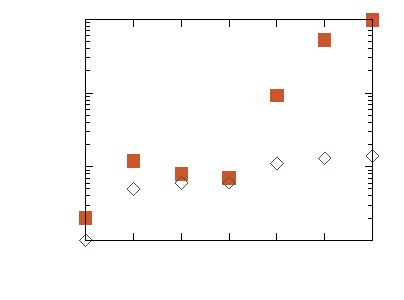
\includegraphics[width={504.00bp},height={144.00bp}]{unhashed-performance-combined}}%
    \gplfronttext
  \end{picture}%
\endgroup
}
%   \caption{Time taken to validate seven increasingly complicated schedules, without final-state guards ($\square$) and with final-state guards ($\diamond$).}%
%   \label{fig:hashed-and-unhashed-performance}
% \end{figure*}

\subsection{Third attempt: using value summaries and final-state guards}
\label{sec:thirdattempt}

Although it was not the case in our worked example, it turns out that when
comparing the predicate expressions that arise in realistic examples, syntactic
equality or near-equality usually suffices. This means that we only need to
resort to solving 3-valued SAT queries as an occasional fallback, so its
performance impact is limited in practice.

Where syntactic methods usually do \emph{not} suffice is for comparing the
guards of register expressions. However, here we can actually avoid the need for
3-valued logic altogether.  We observe that the guards in the \rtlinline|r1|
expressions are simply copied from the expressions for \rtlinline|p2| (which we
abbreviated as $\formY$ in \cref{tab:symbex2}), so rather than writing out the
full expressions in the guards, we can write $\afvar{p2}$ as a shorthand (the
`f' clarifies that it is referring to the \emph{final} value of \rtlinline|p2|).

To make it possible to refer to final values, we need to ensure that once
\rtlinline|p2| has been assigned or used, it is never overwritten. We can
achieve this by enforcing SSA form for predicate assignments. That does not
impose any restrictions on the Vericert user because predicates are only
introduced by internal compiler transformations. SSA form is not needed for
register assignments.

The resultant symbolic states are shown in \cref{tab:third-attempt}. It can
immediately be seen that the expressions have become much shorter. Indeed, the
three queries for validating \rtlinline|r1| become:

\begin{equation}
\begin{aligned}
  \lfalse &\leftrightarrow \satvar{\afvarsmall{p1}} \wedge \satvar{\afvarsmall{p2}} \wedge \neg \satvar{\afvarsmall{p1}}
\\
  \satvar{\afvarsmall{p1}} \wedge \satvar{\afvarsmall{p2}} &\leftrightarrow \satvar{\afvarsmall{p1}} \wedge \satvar{\afvarsmall{p2}} \wedge \satvar{\afvarsmall{p1}}
\\
  \neg(\satvar{\afvarsmall{p1}} \wedge \satvar{\afvarsmall{p2}}) &\leftrightarrow \neg(\satvar{\afvarsmall{p1}} \wedge \satvar{\afvarsmall{p2}})
\end{aligned}
\end{equation}

What is less obvious is that we no longer need 3-valued logic either. This is
because:
\begin{itemize}
\item We can assume that all predicate expressions in the pre-scheduling
  symbolic state are evaluable, because if any were not, the input program would
  fail at run time and we do not need to prove anything about our scheduler.
\item We have already proven, either using syntactic comparison or 3-valued
  logic, that the predicate expressions in the post-scheduling symbolic state
  are equivalent to those in the pre-scheduling state, which means that they too
  must be evaluable.
\item The guards in the register expressions only refer to these expressions --
  they cannot include unsafe expressions like division or pointer comparison --
  and so they must also be evaluable.
\item It therefore suffices to use 2-valued logic to compare the guards.
\end{itemize}

\begin{table}
  \centering
  \captionabove{Third attempt: using value summaries and final values in guards.}\label{tab:third-attempt}
  \begin{tabular}{r|l|l}
    \toprule
    & \textbf{Pre-scheduling symbolic state} & \textbf{Post-scheduling symbolic state} \\ \midrule
    $\text{\rtlinline|r1|}$ & $\begin{cases}
                                 \avar{r2} + 2,&\text{if } \afvar{p1} \land \afvar{p2}\\
                                 \avar{r1},&\text{if } \neg(\afvar{p1} \land \afvar{p2})\\
                               \end{cases}$
    & $\begin{cases}
         1 \aadd 2,&\text{if } \afvar{p1} \land \afvar{p2} \land \neg \afvar{p1}\\
         \avar{r2} + 2,&\text{if } \afvar{p1} \land \afvar{p2} \land \afvar{p1}\\
         \avar{r1},&\text{if } \neg(\afvar{p1} \land \afvar{p2})\\
       \end{cases}$ \\ \midrule
    $\text{\rtlinline|r2|}$ & $\begin{cases}
                                 1,&\text{if } \neg\afvar{p1}\\
                                 \avar{r2},&\text{if } \afvar{p1}\\
                               \end{cases}$ & $\begin{cases}
                                                 1,&\text{if } \neg\afvar{p1}\\
                                                 \avar{r2},&\text{if } \afvar{p1}\\
                                               \end{cases}$
    \\ \midrule
    $\text{\rtlinline|p2|}$ & $\syniteformulans{\avar{p1}}{\avar{r2} \aeq 0}{\avar{p2}}$ & $\syniteformulaaligned{\avar{p1}}{(\syniteformulans{\neg\avar{p1}}{1 \aeq 0}{\avar{r2} \aeq 0})}{\avar{p2}}$\\
    \bottomrule
  \end{tabular}
\end{table}

% These can be checked directly using a SAT solver without requiring
% three-valued logic.  This is because we can assume that all of the predicates
% in the input symbolic state are evaluable, because otherwise the input program
% would contain undefined behaviour.  The equivalence check between symbolic
% expressions associated with predicates uses three-valued logic to ensure that
% the output predicates are also evaluable given that the input predicates were
% evaluable, and that they will evaluate to the same Boolean value.  Finally,
% because guards inside of value summaries are only expressed in terms of
% \emph{final} values of predicates, only Boolean evaluation semantics are
% needed.

%The $\diamond$ data points in \cref{fig:hashed-and-unhashed-performance} show the performance of the equivalence check when predicate expressions are compared using syntactic equality and register expressions are compared via 2-valued SAT solving. We see that it is several orders of magnitude faster.

\subsection{Handling overwritten expressions}%
\label{sec:handling-discarded-expressions}

There is an additional subtlety that needs to be handled: the possibility that
the scheduler introduces undefined behaviour. Consider the following example,
due to \textcite{tristan08_formal_verif_trans_valid}.

\begin{center}
\begin{tikzpicture}
\node (initial) {\begin{minipage}{0.3\linewidth}
\begin{rtllisting}
r3 := r2 + 4;
\end{rtllisting}
\end{minipage}};
\node[right=2cm of initial] (scheduled) {
  \begin{minipage}{0.3\linewidth}
\begin{rtllisting}
r3 := 5/r1;
r3 := r2 + 4;
\end{rtllisting}
  \end{minipage}
};
\draw[-{Latex[length=3mm]}] (initial) -- node [below] {scheduling}
($(scheduled.west)-(0.5,0)$);
\end{tikzpicture}
\end{center}

Symbolic execution yields identical pre- and post-scheduling results, namely
$\text{\rtlinline|r3|} \mapsto \avar{r2} + 4$. Despite this, the schedule is
invalid because the post-scheduling block only executes correctly when
\rtlinline|r1| is nonzero.  To detect and forbid such cases, we follow
\citeauthor{tristan08_formal_verif_trans_valid} and keep track of all the
expressions that are evaluated into a register or memory location. We shall call
this the \emph{encountered expression
  set}.\footnote{\citeauthor{tristan08_formal_verif_trans_valid} simply called
  them `constraints'.} For example, the encountered expressions of the
pre-scheduling block above includes only $\avar{r2} + 4$, but the
post-scheduling block's also includes $5/\avar{r1}$. Because the encountered set
has grown, we deem the schedule invalid.

% \begin{figure}
% \centering
% \begin{tikzpicture}
% \node (initial) {\begin{minipage}{0.2\linewidth}
% \begin{rtllisting}
% r3 := r2 + 4;
% \end{rtllisting}
% \end{minipage}};
% \node[right=2cm of initial] (scheduled) {
%   \begin{minipage}{0.2\linewidth}
% \begin{rtllisting}
% r3 := 5/r1;
% r3 := r2 + 4;
% \end{rtllisting}
%   \end{minipage}
% };
% \node[below=1cm of initial] (initial abstract) {$\text{\rtlinline|r3|} \mapsto
%   \avar{r2} + 4$};
% \path (initial abstract) -| node (scheduled abstract) {$\text{\rtlinline|r3|} \mapsto
%   \avar{r2} + 4$} (scheduled);
% \node[left=1cm of initial abstract] (initial encountered) {$\set{\avar{r2} \aadd 4}$};
% \node[right=1cm of scheduled abstract] (scheduled encountered) {$\set{5 \adiv \avar{r1}, \avar{r2} \aadd 4}$};
%   \draw[-{Latex[length=3mm]}] (initial) -- node [below] {scheduling}
%   ($(scheduled.west)-(0.5,0)$);
%   \draw[-{Latex[length=3mm]}] (initial) -- node[align=center,right] {symbolic \\ execution} (initial abstract);
%   \draw[-{Latex[length=3mm]}] (scheduled) -- node[align=center,left] {symbolic
%     \\ execution} (scheduled abstract);
% \draw[-{Latex[length=3mm]}] (initial) -- node[align=center,above left] {encountered
%   \\ expressions} (initial encountered);
% \draw[-{Latex[length=3mm]}] (scheduled) -- node[align=center,above right] {encountered
%   \\ expressions} (scheduled encountered);
% \end{tikzpicture}
% \caption{Example of symbolic execution where even though the symbolic states are
%   identical, the behaviours could be different because the scheduled code needs
%   \rtlinline|r1| to be non-zero.}%
% \label{fig:example-symb-execution-with-division}
% \end{figure}

In order to use \citeauthor{tristan08_formal_verif_trans_valid}'s approach with
hyperblocks, it needs extending to handle predicated instructions. The obvious
way to do this is to generate the encountered expressions for each predicated
instruction in the same way that we perform symbolic execution, which is
essentially to treat \rtlinline{p => r := e} as if it is the non-predicated
instruction \rtlinline{r := p?e:r}.  However, this approach leads to too many
unnecessary constraints being imposed on the scheduler, leaving it unable to
reorder some instructions that have only benign WAW dependencies. To see this,
consider the following example.
\begin{center}
\begin{tikzpicture}
\node (initial) {\begin{minipage}{0.3\linewidth}
\begin{rtllisting}
p1 => r1 := 1;
!p1 => r1 := 2;
\end{rtllisting}
\end{minipage}};
\node[right=2cm of initial] (scheduled) {
  \begin{minipage}{0.3\linewidth}
\begin{rtllisting}
!p1 => r1 := 2;
p1 => r1 := 1;
\end{rtllisting}
  \end{minipage}
};
\draw[-{Latex[length=3mm]}] (initial) -- node [below] {scheduling}
($(scheduled.west)-(0.5,0)$);
\end{tikzpicture}
\end{center}
When performing symbolic execution on
the pre-scheduling block, we encounter the pair of
expressions
$\synite{\afvar{p1}}{1}{\avar{r1}}$
% $\set{(\afvar{p1}, 1), (\neg\afvar{p1}, \avar{r1})}$
and
$\synite{\neg\afvar{p1}}{2}{\synite{\afvar{p1}}{1}{\avar{r1}}}$,
% $\set{(\afvar{p1}, 1), (\neg\afvar{p1}, 2)}$
but on the
post-scheduling block we encounter
$\synite{\neg\afvar{p1}}{2}{\avar{r1}}$
% $\set{(\neg\afvar{p1}, 2), (\afvar{p1}, \avar{r1})}$
and
$\synite{\afvar{p1}}{1}{\synite{\neg\afvar{p1}}{2}{\avar{r1}}}$;
% $\set{(\neg\afvar{p1}, 2), (\afvar{p1}, 1)}$
these two pairs
are not equivalent, so this (correct) schedule cannot be validated.

Instead, for the purposes of calculating encountered expressions, our approach
is to treat \rtlinline{p => r := e} as the instruction%
\rtlinline{r := p?e:}$\bullet$, where $\bullet$ is a dummy expression
representing the absence of an assignment. Now the set of encountered
expressions is
$\{\synite{\afvar{p1}}{1}{\bullet}, \synite{\neg\afvar{p1}}{2}{\bullet}\}$
%$\set{\set{(\afvar{p1}, 1),
%    (\neg\afvar{p1}, \bullet)}, \set{(\neg\afvar{p1}, 2), (\afvar{p1}, \bullet)}}$
both pre- and post-scheduling, so validation can be completed.

%This approach is borrowed from the concept of \emph{constraints} by
%\textcite[]{tristan08_formal_verif_trans_valid}.  Constraints are a set of
%intermediate symbolic states that were associated with a register or memory
%location, which give a set of well-defined symbolic states.  The constraints of
%the scheduled code must then be a subset of the constraints of the input code,
%to check that no additional operations were erroneously introduced by the
%scheduler.  Predicated instructions can update the state partially instead, and
%can rearrange WAW conflicts, with the consequence that partial updates to a
%symbolic state can come in a different order.  This may produce different
%intermediate states that cannot be compared anymore.
%\Cref{fig:storing-intermediate-instructions} shows an example of this, where a
%WAW can be ignored because of the predicates, which leads to partial updates
%being applied in a different order.  The first method shown is storing
%intermediate states in the set of constraints, which differ and therefore cannot
%be compared.  Instead, a set of \emph{encountered expressions} is produced.
%Each instruction used to update the state is converted to a symbolic
%expression, and is combined with a trivially evaluable symbolic expression to
%produce a value summary describing the partial update.  In this case we just
%pick an arbitrary base register $\avar{r}$ which will always be evaluable.

%\begin{figure}
%\centering
%\begin{tikzpicture}
%\node (initial) {\begin{minipage}{0.3\linewidth}
%\begin{rtllisting}
%p1 & p2 => r1 := 1;
%!p1 & p2 => r1 := 2;
%\end{rtllisting}
%\end{minipage}};
%\node[right=2cm of initial] (scheduled) {
%  \begin{minipage}{0.3\linewidth}
%\begin{rtllisting}
%!p1 & p2 => r1 := 2;
%p1 & p2 => r1 := 1;
%\end{rtllisting}
%  \end{minipage}
%};
%\node[above=1cm of initial] (initial abstract) {$\left\{\,
%  \begin{aligned}
%      &\{\, (\afvar{p1} \land \afvar{p2},
%  1), (\neg(\afvar{p1} \land \afvar{p2}),
%  \avar{r1}) \,\},\\
%      &\left\{\,
%        \begin{aligned}
%          &(\afvar{p1} \land \afvar{p2},
%          1), (\neg\afvar{p1} \land \afvar{p2}, 2), \\
%          &(\neg \afvar{p2},
%          \avar{r1})
%        \end{aligned}\,\right\}
%    \\
%  \end{aligned}
% \,\right\}$};
%\path (initial abstract) -| node (scheduled abstract) {$\left\{\,
%  \begin{aligned}
%      &\{\, (\neg\afvar{p1} \land \afvar{p2}, 2), (\neg(\neg\afvar{p1} \land \afvar{p2}),
%  \avar{r1}) \,\},\\
%      &\left\{\,
%        \begin{aligned}
%          &(\afvar{p1} \land \afvar{p2},
%          1), (\neg\afvar{p1} \land \afvar{p2}, 2), \\
%          &(\neg \afvar{p2},
%          \avar{r1})
%        \end{aligned}\,\right\}
%    \\
%  \end{aligned}
% \,\right\}$} (scheduled);
%  \node [below=1cm of initial] (initial ideally) {$
%    \left\{\,\begin{aligned}
%               &\{\,(\afvar{p1} \land \afvar{p2}, 1), (\neg(\afvar{p1} \land \afvar{p2}), \avar{r})\,\},\\
%               &\{\,(\neg\afvar{p1} \land \afvar{p2}, 2), (\neg(\neg\afvar{p1} \land \afvar{p2}), \avar{r})\,\}\\
%    \end{aligned}\,\right\}
%    $};
%  \path (initial ideally) -| node (scheduled ideally) {$
%    \left\{\,\begin{aligned}
%               &\{\,(\neg\afvar{p1} \land \afvar{p2}, 2), (\neg(\neg\afvar{p1} \land \afvar{p2}), \avar{r})\,\},\\
%               &\{\,(\afvar{p1} \land \afvar{p2}, 1), (\neg(\afvar{p1} \land \afvar{p2}), \avar{r})\,\}\\
%    \end{aligned}\,\right\}
%    $} (scheduled);
%  \draw[-{Latex[length=3mm]}] (initial) -- node [below] {scheduling}
%  ($(scheduled.west)-(0.5,0)$);
%  \draw[-{Latex[length=3mm]}] (initial) -- node[align=center,left] {intermediate
% \\ states} (initial abstract);
%  \draw[-{Latex[length=3mm]}] (scheduled) -- node[align=center,right] {intermediate
% \\ states} (scheduled abstract);
%  \draw[-{Latex[length=3mm]}] (scheduled) -- node[align=center,right]
%  {encountered \\ expressions} (scheduled ideally);
%  \draw[-{Latex[length=3mm]}] (initial) -- node[align=center,left]
%  {encountered \\ expressions} (initial ideally);
%  \path (initial abstract) -- node {$\not\gtrsim$} (scheduled abstract);
%  \path (initial ideally) -- node {$\gtrsim$} (scheduled ideally);
%\end{tikzpicture}
%\caption{Showing na\"ive storing of intermediate states compared to only storing the partial updates to the states by only storing the symbolic instructions.  In the encountered expressions, $\avar{r}$ is a dummy base register that is trivially evaluable, and it is only used to fill out the expression to make it a valid value summary.}%
%\label{fig:storing-intermediate-instructions}
%\end{figure}

\subsection{Formalising the symbolic state and symbolic execution}
\label{sec:algorithm-symbolic-execution}

%To validate a schedule, we need to be able to compare the symbolic
%configurations before and after scheduling.  That is, the register, predicate,
%and memory expressions in the input configuration must all be equivalent to the
%corresponding expressions in the output configuration. The scheduled block must
%also terminate in the same manner as the original block; this is checked by
%confirming that the two exit expressions are equivalent. Finally, the scheduled
%block must not introduce any new possibilities for runtime errors; this is
%checked by comparing the fifth components.  The next few sections will describe
%the structure of the symbolic expressions by working through an example symbolic
%execution.

The previous sections gave an informal overview of the structure of the symbolic
state and the validation algorithm.  This section will give formal definitions
of these concepts.

\paragraph{Symbolic states}
\Cref{fig:abstract-components} defines the symbolic states that symbolic
execution produces. Several components make use of value summaries (as explained
in \cref{sec:value_summaries}), so we define the value summary $\predicated{t}$
as a set of terms of type $t$, each paired with a Boolean guard of type
$\guardtype$. Henceforth, we shall sometimes write value summaries explicitly as
a set of (guard, value) pairs.

A symbolic state $\symbstate$ is made up of five components, the main three
being: a register map $\forestregset{\symbstate}$ that assigns an arithmetic
expression (as a value summary) to each register, a predicate map
$\forestpredset{\symbstate}$ that assigns a Boolean expression to each
predicate, and an expression $\forestmem{\symbstate}$ for the contents of memory
(again as a value summary).  We also need symbolic execution to track how
control exits the block (to make sure that it does so in the same way after
scheduling), so $\forestexit{\symbstate}$ stores a value summary that evaluates
to the instruction that is executed to exit the block (or to `None' if the block
hasn't finished yet). Finally, $\constraints{\symbstate}$ tracks the set of
encountered expressions, as motivated in
\cref{sec:handling-discarded-expressions}.

% \JW{Actually, I wonder
%  if we can manage without the distinction between symbolic states and symbolic
%  configurations now. Just say that a symbolic state has five components,
%  done. The distinction might have been helpful in the previous subsection when
%  we were trying to build things up slowly, but now we're giving all the gory
%  details, I don't think we need to distinguish them.}

%Registers, the memory and exit expressions are formulated as different value
%summaries, whereas the set of encountered expressions are a set of value
%summaries for memories or for registers.  Finally, predicates are defined in
%terms of predicate expressions $\predexprtype$ which are logical expressions in
%terms of initial predicates and arithmetic operations, which in turn are
%expressed in terms of initial registers and the initial memory.

\begin{figure*}
  \centering
  \begin{tabular}{rr@{~}r@{~}ll}~
    \llabel{arithmetic expressions} & $\exprtype$     & ::= & $\base{\regtype}$ & \rlabel{initial value of register} \\
    & & | & $\anload{\memexprtype}{\exprtype}$ & \rlabel{load from memory} \\
    & & | & $\exprtype \mathbin{\exproptype} \exprtype$ & \rlabel{binary arithmetic operation} \\
    \llabel{memory expressions} & $\memexprtype$ & ::= & $\emptyabstrmem$ & \rlabel{initial contents of memory} \\
    & & | & $\anstore{\memexprtype}{\exprtype}{\exprtype}$ & \rlabel{updated memory} \\
    \llabel{predicate expressions} & $\predexprtype$ & ::= & $\base{\predvartype}$ |
                                                        $\neg \base{\predvartype}$ & \rlabel{initial value of predicate}\\
    & & | & $\exprtype \mathbin{\condoptype} \exprtype$ |
                                                        $\neg (\exprtype
                                                        \mathbin{\condoptype} \exprtype)$ & \rlabel{binary conditional operation} \\
    & & | & $\ltrue$ | $\lfalse$ | $\predexprtype \land \predexprtype$ | $\predexprtype \lor \predexprtype$ & \rlabel{true, false, and, or} \\
    \llabel{value summaries} & $\predicated{t}$ & = &
    %$\listt{(t~\text{if}~\pred)}$
    $\settype{\guardtype \times t}$
          & \rlabel{select an element of $t$ according} \\
    & & & & \rlabel{to which predicate holds} \\
    \llabel{symbolic states} & $\forestregset{\symbstate} \in \forestregset{\symbstatetype}$ & $=$ & $\regtype \rightarrow
                                                        \predicated{\exprtype}$
                                                                               &
                                                                                 \rlabel{expressions for registers} \\
                   & $\forestpredset{\symbstate} \in \forestpredset{\symbstatetype}$ & $=$ & $\predvartype \rightarrow
                           \predexprtype$ & \rlabel{expressions for predicates} \\
                   & $\forestmem{\symbstate} \in \forestmem{\symbstatetype}$ & $=$ &
                                                          $\predicated{\memexprtype}$ & \rlabel{contents of memory} \\
                       & $\forestexit{\symbstate} \in \forestexit{\symbstatetype}$ & $=$ & $\predicated{\optiontype{\cfinstrtype}}$ &
                                                                            \rlabel{instruction to exit block} \\
                   & $\constraints{\symbstate} \in \constraints{\symbstatetype}$ & $=$ & $\settype{\predicated{\exprtype
                                                     + \memexprtype}}$
                                    & \rlabel{set of encountered expressions}\\
  \end{tabular}
  \caption{Syntax of symbolic states.} %
  \label{fig:abstract-components}
\end{figure*}

%To formalise discarded sets properly, we extend the symbolic states we have seen
%so far into \emph{symbolic configurations}. A symbolic configuration consists of
%a symbolic state plus two additional components:
%
%\begin{itemize}
%\item an expression that evaluates to the control-flow instruction that exits
%  the block (or to None if execution hasn't yet finished), and
%
%\item a set of discarded expressions.
%\end{itemize}
%
%The purpose of the first component is to track the manner in which control exits
%the block -- this is another behaviour that we must check that the schedule
%preserves.  Next, the set of discarded expressions is used to check that the
%discarded expressions of the output are a subset of the discarded expressions of
%the input.

\paragraph{Constructing symbolic states}
The expressions are constructed using a function which updates the symbolic
expressions assigned for each resource.  A core function used to update value
summaries is the coalescing union operator $\predicatedappend{q}{}{}$
\cite{sen15_multis}, which conjoins $\neg q$ to each guard in its left operand
and $q$ to each guard in its right operand:
\begin{equation}
\begin{aligned}
  & \predicatedappend{q}{}{} \in \predicated{\mathbb{X}} \rightarrow \predicated{\mathbb{X}} \rightarrow \predicated{\mathbb{X}} \\
  & \predicatedappend{q}{X_1}{X_2} \defeq \{ (\neg q \land \guard, v) \mid (\guard,v) \in X_1 \} \cup \{ ( q \land \guard, v) \mid (G,v) \in X_2 \}
\end{aligned}
\end{equation}

To turn a value summary back into a Boolean formula, we use the following
operation, where $g$ expands gates into predicate expressions:
\begin{equation}
\begin{aligned}
    & {\land} \in \predicated{\predexprtype} \rightarrow \predexprtype \\
    & {\land}\set{(\guard_1, \predexpr_1), \ldots, (\guard_n, \predexpr_n)} \defeq (g(\guard_1) \rightarrow \predexpr_1) \land \dots \land (g(\guard_n) \rightarrow \predexpr_n)
    \end{aligned}
  \end{equation}

  It is also useful to have an applicative interface for value summaries, so
  that when we have value summaries of functions and of inputs, we can obtain a
  value summary of outputs:
\begin{equation}\label{eq:applicative}
  \begin{aligned}
    &\applic \in \predicated{\mathbb{X} \rightarrow \mathbb{Y}} \rightarrow \predicated{\mathbb{X}}
    \rightarrow \predicated{\mathbb{Y}}\\
    &F \applic X \defeq \set[(\guard \land \guard',
      f(x))]{(\guard, f) \in F, (\guard', x) \in X}
  \end{aligned}
\end{equation}

Following \textcite{sen15_multis}, we simplify value summaries as they are built
up, so as to keep their size from exploding: coalescing two elements
$(\guard, v)$ and $(\guard', v')$ where $v = v'$ into a single element
$(\guard \lor \guard', v)$, and removing elements $(\guard, v)$ whenever
$\guard \leftrightarrow \lfalse$.

%We then define a version of the coalescing union operator for
%updating value summaries with a particular predicate that was encountered.

\paragraph{Symbolic execution}
The symbolic execution of instruction $\instr$ is performed by the $\update$
function. It takes the current symbolic state $\symbstate$ and produces an
updated one. It also takes an `enabled' predicate $q$, which is conjoined with
the current instruction's guard; it ensures that after an exit instruction is
taken, any subsequent instructions are nullified. So, whenever an exit
instruction is encountered, the enabled predicate is conjoined with the negation
of the exit instruction's guard.

\begin{figure}
\[
  \begin{array}{ll}
%    &\updateforest(\asgninstr[p]{d}{r_1 \cadd r_2}, q, \symbstate) \\
%    &\qquad\defeq
%      \at{\forestregset{\symbstate}}{d \mapsto (\predicatedappend{p \land
%      q}{\at{\symbstate}{d}}{\set[(p_1 \land p_2, v_1 \aadd v_2)]{((p_1, v_1), (p_2, v_2)) \in (\at{\symbstate}{r_1} \times \at{\symbstate}{r_2}) }})}\\
%    &\qquad \quad\  \constraints{\symbstate} \mapsto \constraints{\symbstate} \cup \set{ \set[(p \land q
%      \land p_1 \land p_2, v_1 \aadd v_2)]{((p_1, v_1), (p_2, v_2)) \in
%      (\at{\symbstate}{r_1} \times \at{\symbstate}{r_2}) } } \\[1ex]
%      %
    \update\ (\asgninstr[\guard]{\mrtl{r}}{\mrtl{r1} \cadd \mrtl{r2}})\ (q, (\forestregset{\symbstate}, \forestpredset{\symbstate}, \forestmem{\symbstate}, \forestexit{\symbstate}, \constraints{\symbstate})) & \text{\rlabel{arithmetic operation}} \\
    %&\quad\defeq
   %   \text{let}~\phi = \set[(\guard_1 \land \guard_2, v_1 \aadd v_2)]{((\guard_1, v_1), (\guard_2, v_2)) \in (\atforestregs{\symbstate}{r1} \times \atforestregs{\symbstate}{r2}) }~\text{in}\\
       \quad \defeq \letin{\phi = \set{(\ltrue, (\mathtt{+}))} \applic \atforestregs{\symbstate}{\mrtl{r1}} \applic \atforestregs{\symbstate}{\mrtl{r2}}}\\
      \quad \quad\ \letin{\forestregset{\symbstate}' = \at{\forestregset{\symbstate}}{\mrtl{r} \mapsto (\predicatedappend{\guard \land
      q}{\at{\forestregset{\symbstate}}{\mrtl{r}}}{\phi})}}\\
    \quad \quad\  \letin{\constraints{\symbstate}' =
      \constraints{\symbstate} \cup \set{ \predicatedappend{\guard \land
      q}{\set{ (\ltrue, \bullet) }}{\phi} }} \\
      \quad \quad\ (q, (\forestregset{\symbstate}', \forestpredset{\symbstate},
        \forestmem{\symbstate}, \forestexit{\symbstate},
        \constraints{\symbstate}'))
%      &\quad \quad\ (\at{\forestregset{\symbstate}}{\mrtl{r} \mapsto (\predicatedappend{\guard \land
%      q}{\at{\forestregset{\symbstate}}{\mrtl{r}}}{\phi})}, \forestpredset{\symbstate}, \forestmem{\symbstate}, \forestexit{\symbstate}, \constraints{\symbstate} \cup \set{ \predicatedappend{\guard \land
%      q}{\set{ (\ltrue, \bullet) }}{\phi} })
      \\[1ex]
      %
    \update\ (\exitinstr[\guard]{\cfinstr})\ (q, (\forestregset{\symbstate}, \forestpredset{\symbstate}, \forestmem{\symbstate}, \forestexit{\symbstate}, \constraints{\symbstate}))  & \text{\rlabel{exit instruction}} \\
    \quad\defeq \letin{\forestexit{\symbstate'} = \predicatedappend{\guard \land
      q}{\forestexit{\symbstate}}{\set{(\ltrue, \some{\cfinstr})}}}\\
    \quad\quad \left( q  \land \neg G , \left(\forestregset{\symbstate}, \forestpredset{\symbstate}, \forestmem{\symbstate}, \forestexit{\symbstate'},
      \constraints{\symbstate}\right)\right)\\[1ex]
    %
    \update\ (\asgninstr[\guard]{\mrtl{p}}{\mrtl{r1} \ceq \mrtl{r2}})\ (q, (\forestregset{\symbstate}, \forestpredset{\symbstate}, \forestmem{\symbstate}, \forestexit{\symbstate}, \constraints{\symbstate})) & \text{\rlabel{predicate assignment}}\\
    \quad\defeq
      %\text{let}~\phi = \land\set[(\guard \land q \land \guard_1 \land \guard_2 \rightarrow v_1 \aeq v_2)]{((\guard_1, v_1), (\guard_2, v_2)) \in (\atforestregs{\symbstate}{r1} \times \atforestregs{\symbstate}{r2})}~\text{in}\\
      \letin{\phi = \land(\set{(G \land q, (\ceq))} \applic \atforestregs{\symbstate}{\mrtl{r1}} \applic \atforestregs{\symbstate}{\mrtl{r2}})}\\
      \quad \quad\ \letin{\forestpredset{\symbstate'} = \at{\forestpredset{\symbstate}}{\mrtl{p} \mapsto
      (\phi \land (\neg (\guard \land q) \rightarrow
                \atforestpreds{\symbstate}{\mrtl{p}})
      )}}\\
                \quad \quad\ (q, (\forestregset{\symbstate}, \forestpredset{\symbstate'}, \forestmem{\symbstate}, \forestexit{\symbstate}, \constraints{\symbstate}))
                \end{array}
                \]
                \caption{Symbolic execution of selected instructions}
                \label{fig:alpha}
\end{figure}

In \cref{fig:alpha}, we show three important cases of $\update$: symbolically
executing an arithmetic operation, an exit instruction, and a predicate
assignment. To symbolically execute a whole hyperblock
(denoted~$\symbolic{\cdot}$), we run $\update$ on each instruction in turn,
threading the symbolic state through, starting from the empty symbolic state
(denoted $\varnothing$):
\begin{equation}\label{eq:symex_block}
  \symbolic{[i_1; i_2; \dots ; i_n]} \defeq \update\ i_n\
  (\dots (\update\ i_2\ (\update\ i_1\ (\ltrue, \varnothing)))\dots)
\end{equation}


\paragraph{Comparing symbolic states}
After symbolically executing the \rtlblock{} and \rtlpar{} blocks, we obtain two
symbolic states, $\symbstate$ and $\symbstate'$. We wish to show that
$\symbstate'$ is a \emph{symbolic refinement} of $\symbstate$ (written
$\symbstate\gtrsim\symbstate'$), and we do so by component-wise comparison, as
shown in \cref{eq:symbolic_refinement} and explained below.

\begin{equation}\label{eq:symbolic_refinement}
  \inferrule{%
    \compare{}{\forestregset{\symbstate}}{\forestregset{\symbstate}'} \and
    {\forestpredset{\symbstate}} = {\forestpredset{\symbstate}'} \lor
    {\forestpredset{\symbstate}} \approx_{\mathrm{3v}} {\forestpredset{\symbstate}'}
    \and
    \compare{}{\forestmem{\symbstate}}{\forestmem{\symbstate}'} \and
    \compare{}{\forestexit{\symbstate}}{\forestexit{\symbstate}'} \and
    {\constraints{\symbstate}}\gtrsim{\constraints{\symbstate}'}
  }{\symbstate\gtrsim\symbstate'}
\end{equation}

The core comparison operation that we rely upon is between two value summaries,
written $\compare{\predicated{t}}{}{}$. Whenever a value appears in both value
summaries, we check that its guards are equivalent (via a SAT query), and
whenever a value appears in just one value summary, we check that its guard is
equivalent to False (again via SAT query). This approach suffices for the
register maps
($\compare{}{\forestregset{\symbstate}}{\forestregset{\symbstate}'}$), the
memory maps ($\compare{}{\forestmem{\symbstate}}{\forestmem{\symbstate}'}$), and
the exit expressions
($\compare{}{\forestexit{\symbstate}}{\forestexit{\symbstate}'}$). For the
predicate maps, we first attempt to show syntactic equality
(${\forestpredset{\symbstate}} = {\forestpredset{\symbstate}'}$). If this fails,
we fall back to using a slow but reliable equivalence check with a 3-valued
solver
(${\forestpredset{\symbstate}} \approx_{\mathrm{3v}}
{\forestpredset{\symbstate}'}$). Finally, for the encounted expressions sets, we
write ${\constraints{\symbstate}}\gtrsim{\constraints{\symbstate}'}$ to mean
that every expression in $\constraints{\symbstate}'$ has an equivalent in
$\constraints{\symbstate}$.
% \JW{Good. We need a name for the $\symbstate\gtrsim\symbstate'$ relation. The
% symmetric version could have been called something like `symbolic
% equivalence', as it is an equivalence between symbolic states. But we need an
% anti-symmetric version. Possibly `symbolic refinement'? That is, we could say
% that $\symbstate'$ `symbolically refines' $\symbstate$? And if we lift this
% from symbolic states up to blocks, we could say that
% $\symbolic{B}\gtrsim\symbolic{P}$ can be read as `$P$ symbolically refines
% $B$'. Then the big correctness theorem can be stated concisely and precisely
% as: ``if $P$ symbolically refines $B$, then there is a forward simulation from
% $B$ to $P$.'' Or even:
%   \[
%   (\gtrsim) \subseteq (\curly)
%   \]
%   }



%\subsubsection{Equivalence checking overview}

% \begin{figure*}
%   \centering
%   \begin{tikzpicture}[>=Latex,shorten >=1pt,node distance=5mm and 25mm,%
%     language/.style={very thick,draw,fill=MistyRose,font={\sffamily\bfseries}},%
%     translation/.style={very thick,draw,ellipse,fill=Orchid!40,font={\sffamily\bfseries}},%
%     check/.style={very thick,draw,rounded rectangle,fill=DarkSeaGreen!50,font={\sffamily\bfseries\boldmath}}]
%     \node[ir,align=center] (rtlblock) {\rtlblock \\ hyperblock};
%     \node[pass,right=of rtlblock] (scheduling) {Scheduling};
%     \node[ir,right=of scheduling,align=center] (rtlpar) {\rtlpar \\ hyperblock};
%     \node[pass,align=center,below=of rtlblock] (symba) {Symbolic\\Execution};
%     \node[pass,align=center,below=of rtlpar] (symbb) {Symbolic\\Execution};
%     \node[ir,below=0.75 of symba] (abstrinstra) {$\forestregset{\symbstate},
%       \forestmem{\symbstate}$};
%     \node[ir,left=0.5 of symbb] (constrb) {$\constraints{\symbstate}$};
%     \node[ir,right=0.5 of symba] (constra) {$\constraints{\symbstate}$};
%     \node[ir,below=0.25 of constra] (abstrexita) {$\forestexit{\symbstate}$};
%     \node[ir,below=0.25 of abstrinstra] (abstrpreda) {$\forestpredset{\symbstate}$};
%     \node[above left=0.1 of abstrinstra,xshift=1cm,inner sep=0] (abstrlabela)
%     {$\foreststate{\symbstate}$};
%     \node[ir,below=0.75 of symbb] (abstrinstrb) {$\forestregset{\symbstate}, \forestmem{\symbstate}$};
%     \node[ir,below=0.25 of constrb] (abstrexitb) {$\forestexit{\symbstate}$};
%     \node[ir,below=0.25 of abstrinstrb] (abstrpredb) {$\forestpredset{\symbstate}$};
%     \node[above left=0.1 of abstrinstrb,xshift=1cm,inner sep=0] (abstrlabelb)
%     {$\foreststate{\symbstate}$};
%     \begin{pgfonlayer}{background}
%       \node[ir,fit={(abstrinstra)(abstrpreda)(abstrlabela)}]
%       (abstra) {};
%       \node[ir,fit={(abstrinstrb)(abstrpredb)(abstrlabelb)}]
%       (abstrb) {};
%     \end{pgfonlayer}
% %    \node[check] at ($(constra)!0.5!(constrb)$) (checkconstr) {$\sqsupseteq$};
%     \node[check] at ($(constra)!0.5!(constrb)$) (checkconstr) {SAT: $\gtrsim$};
%     \node[check] at ($(abstrinstra)!0.5!(abstrinstrb)$) (checksata) {SAT: $\approx$};
%     \node[check] at ($(abstrexita)!0.5!(abstrexitb)$) (checksatb) {SAT: $\approx$};
%     \node[check] at ($(abstrpreda)!0.5!(abstrpredb)$) (checksmt) {$=$ / SMT: $\approx_{\mathrm{3v}}$};
%     \draw[ed] (rtlblock) -- (scheduling);
%     \draw[ed] (scheduling) -- (rtlpar);
%     \draw[ed] (rtlblock) -- (symba);
%     \draw[ed] (symba) -- (abstra);
%     \draw[ed] (symbb) -- (abstrb);
%     \draw[ed] (rtlpar) -- (symbb);
%     \draw[ed] (symba) -- (constra);
%     \draw[ed] (symbb) -- (constrb);
%     \draw[ed] (symbb) -- (abstrexitb);
%     \draw[ed] (symba) -- (abstrexita);
%     \draw[ed] (constra) -- (checkconstr);
%     \draw[ed] (constrb) -- (checkconstr);
%     \draw[ed] (abstrinstra) -- (checksata);
%     \draw[ed] (abstrinstrb) -- (checksata);
%     \draw[ed] (abstrexita) -- (checksatb);
%     \draw[ed] (abstrexitb) -- (checksatb);
%     \draw[ed] (abstrpreda) -- (checksmt);
%     \draw[ed] (abstrpredb) -- (checksmt);
%   \end{tikzpicture}
%   \caption{Diagram showing the steps performed by the verified checker to ensure
%     that the scheduled hyperblock is equivalent to the original hyperblock by
%     symbolically executing both programs resulting in a symbolic state
%     $\symbstate$ assigning symbolic expressions to registers
%     $\forestregset{\symbstate}$ to predicated expressions memory expressions
%     $\forestmem{\symbstate}$ and predicate expressions
%     $\forestpredset{\symbstate}$.  In addition to that, there are also exit
%     expression $\forestexit{\symbstate}$ and encountered expressions
%     $\constraints{\symbstate}$ that need to be compared.  Each of these are
%     checked for equivalence using a verified SAT solver or an SMT solvers by
%     reusing the SMTCoq proof checker.\YH{TODO: fix the hierarchy without configuration.} \JW{I suggest a shorter caption, e.g. `Checking equivalence between symbolic states, component by component.'}}%
%   \label{fig:scheduling-steps}
% \end{figure*}

% After having symbolically executed both the \rtlblock{} and \rtlpar{} blocks,
% one needs to compare the two to check if they are equivalent.  In the previous
% sections, the equivalence checks between the different components of the
% symbolic state have already been discussed.  This section will give a formal
% description of the equivalence checking algorithm used. An overview of the
% checking algorithm is shown in \cref{fig:scheduling-steps}.

% Because the scheduler can reorder instructions based on predicates, we need a comparison function that takes into account the logical formulas, and will accept two \abstr{} blocks even though the contents assigned to each register are not exactly the same syntactically, because of the order in which the blocks were evaluated.  In addition to that, the scheduler may have eliminated redundant expressions which need to be handled.  The core comparison operation that needs to be implemented is between two $\predicated{t}$ expressions, where $t$ can be compared syntactically.  Using such a function, defined as $\compare{\predicated{t}}{\cdot}{\cdot} : \predicated{t} \rightarrow \predicated{t} \rightarrow \mono{bool}$, in addition to a syntactic equality between two $\predexprtype$ expressions, which is sufficient in most cases. Finally, a comparison function $\cdot \gtrsim \cdot$ is defined to compare two sets of encountered expressions.  It checks that all the expressions in the output set of encountered expressions have an equivalent expression in the input set, showing that no additional expressions were introduced.

%\begin{equation}
%  \label{eq:4}
%  \compare{\abstr}{a}{b} \defeq \bigwedge
%  \left(\,\begin{aligned}
%    &\forall x\ldotp
%      \compare{\predicated{\abstrexpr}}{\at{\forestregset{a}}{x}}{\at{\forestregset{b}}{x}}\\
%    &\forall x\ldotp {\at{\forestpredset{a}}{x}} = {\at{\forestpredset{b}}{x}}\\
%    &\compare{\predicated{\abstrmem}}{\forestmem{a}}{\forestmem{b}}\\
%    &\compare{\predicated{\cfinstrtype?}}{\forestexit{a}}{\forestexit{b}}\\
%    &\constraints{a} \gtrsim \constraints{b}\\
%  \end{aligned}\,\right)
%\end{equation}

%\YH{TODO: fix the vector notation here too.}

%In the case where the syntactic equality check between two $\predexprtype$ expressions fails, there are looser equivalence checks that could be tried.  The first would be to try to normalise the $\predexprtype$ to be able to catch more cases using a simple syntactic equality.  Otherwise, one can fall back to using a slow but reliable equivalence check using a three-valued SAT solver, which is what was implemented.

%\subsubsection{Summary}
%
%This section formalises the symbolic execution algorithm which was described
%through examples in the previous sections.
%
%\begin{itemize}
%\item We normalise register expressions into \emph{value summaries}, because
%  this reduces the equivalence check to between arithmetic expressions
%  (\rtlinline|A|s and \rtlinline|A'|'s), which can be compared syntactically,
%  and between boolean guards (\rtlinline|G|s and \rtlinline|G'|s), which can be
%  compared using a verified SAT solver.
%\item To account for the possibility of unevaluable expressions, we need to use
%  \rtlinline|option| types when comparing the \rtlinline|A|s and
%  \rtlinline|A'|'s and the \rtlinline|B|s and \rtlinline|B|s. This is not a
%  problem in practice because they tend to be syntactically identical or
%  near-identical.
%\item To avoid the need for three-valued logic when comparing the \rtlinline|G|s
%  and \rtlinline|G|`s, we restrict their form to simple combinations of \rtlinline|p|s and
%  evaluate them in the \emph{final} state (but the \rtlinline|A`s and `B|s are
%  still evaluated in the \emph{initial} state).
%\item So that \rtlinline|p|s can be safely evaluated in the final state, we
%  enforce SSA form on predicates.
%\item Finally, we track "discarded" expressions (following Tristan and Leroy) to
%  ensure that the scheduler does not introduce a runtime failure that is
%  otherwise hidden by overwriting.
%\end{itemize}

\subsection{Defining a Verified Scheduler}

We can now define a verified scheduler using the standard translation
validation approach:

  \begin{equation*}
    \begin{aligned}
      \mathtt{scheduleAndVerify}~\rtlbb \defeq {}&\letin{\rtlpb =
                                           \mathtt{schedule}~\rtlbb}\\
                                         &\synite{\symbolic{\rtlbb}
                                           \gtrsim \symbolic\rtlpb}{\ccok{\rtlpb}}{\ccerror}
    \end{aligned}
  \end{equation*}

\section{Proving the Validator Correct}%
\label{sec:hs:overview-validator-correctness-proof}

In order to prove our validator correct, we need to prove that whenever our
validator deems $\symbolic{\rtlpb}$ to be a symbolic refinement of
$\symbolic{\rtlbb}$, there is indeed a forward simulation from $\rtlbb$ to
$\rtlpb$; that is:
  \begin{equation}
    \symbolic{\rtlbb} \gtrsim \symbolic{\rtlpb} \implies \rtlbb \curly \rtlpb
  \end{equation}

  The natural way to prove $\rtlbb \curly \rtlpb$ is to follow
  \textcite{tristan08_formal_verif_trans_valid} by constructing the chain
  $\rtlbb \curly \symbolic{\rtlbb} \curly \symbolic{\rtlpb} \curly \rtlpb$. In
  order to do this, we need to be able to talk about forward simulations that
  involve not just programs ($\rtlbb$ and $\rtlpb$) but also symbolic states
  ($\symbolic{\rtlbb}$ and $\symbolic{\rtlpb}$). Thus we need a semantics not
  just for blocks (cf. \cref{fig:semantics-of-rtlblock-and-rtlpar}) but also for
  symbolic states.

\subsection{A semantics for symbolic states}

We need a function that takes a symbolic state $\symbstate$ and applies it to an
initial concrete state $\context$. The output is the concrete state $\context'$,
together with the control-flow instruction $\cfinstr$ that is executed to exit
the block. The function is written as
$\sem{}{\context}{\symbstate}{(\context',\cfinstr)}$, and is defined in
\cref{fig:regset-semantics}. It works as follows:


\begin{figure}
  \centering
  \begin{mathpar}
    \inferrule[RegBase]{ }{\semval{r^0}{\atforestregs{\context}{r}}}
    \label{rule:regbase}
    \and
    \inferrule[PredBase]{ }{\sempred{p^0}{\atforestpreds{\context}{p}}}
    \label{rule:predbase}
    \and
    \inferrule[MemBase]{
    }{\semmem{\emptyabstrmem}{\forestmem{\context}}}
    \label{rule:membase}
    \and
    \inferrule[Option]{
    }{\semexit{\some{a}}{a}}
    \label{rule:option}
    \\
%    \inferrule[AOp]{\semvallist{l_{\mathrm{e}}}{l_{\mathrm{v}}} \\
%      \evalop{\mathit{op}}{l_{\mathrm{v}}}{v}}{\semval{\aop{\mathit{op}}{l_{\mathrm{e}}}}{v}}
%    \\
    \inferrule[Op]{
    \semval{e_1}{v_1} \\
    \semval{e_2}{v_2} \\\\
    \evalop{v_1\ \exprop\ v_2}{v}
    }{\semval{e_1\ \exprop\ e_2}{v}}%\qquad
    \label{rule:op}
\and
    \inferrule[Pred]{
    \semval{e_1}{v_1} \\
    \semval{e_2}{v_2} \\\\
    \evalop{v_1\ \condop\ v_2}{\some{b}}
    }{ \sempred{e_1\ \condop\ e_2}{b} }
    \label{rule:pred}
\and
    %sem_mem ctx mexp m' ->
    %sem_value ctx vexp v ->
    %sem_val_list ctx args lv ->
    %Op.eval_addressing (ctx_ge ctx) (ctx_sp ctx) addr lv = Some a ->
    %Memory.Mem.storev chunk m' a v = Some m'' ->
    %sem_mem ctx (Estore vexp chunk addr args mexp) m''
    \inferrule[Store]{
      \semmem{e_1}{m} \\\\
      \semval{e_2}{i} \\
      \semval{e_3}{v}
    }{ \semmem{\anstore{e_1}{e_2}{e_3}}{m[i \mapsto v]} }
    \label{rule:store}
\and
    %
    %sem_mem ctx mexp m' ->
    %sem_val_list ctx args lv ->
    %Op.eval_addressing (ctx_ge ctx) (ctx_sp ctx) addr lv = Some a ->
    %Memory.Mem.loadv chunk m' a = Some v ->
    %sem_value ctx (Eload chunk addr args mexp) v
    \inferrule[Load]{
      \semmem{e_1}{m} \\\\
      \semval{e_2}{i}
    }{\semval{\anload{e_1}{e_2}}{\loadv{m}{i}}}
    \label{rule:load}
\and
    \inferrule[PredAndTrue]{ \sempred{\predexpr_1}{\booleantrue} \\\\
      \sempred{\predexpr_2}{\booleantrue} }{ \sempred{\predexpr_1 \land
        \predexpr_2}{\booleantrue} }
        \label{rule:predandtrue}
    \and
    \inferrule[PredAndFalse1]{ \sempred{\predexpr_1}{\booleanfalse} }{ \sempred{\predexpr_1 \land
        \predexpr_2}{\booleanfalse} }
        \label{rule:predandfalse1}
\and
    \inferrule[PredAndFalse2]{ \sempred{\predexpr_2}{\booleanfalse} }{ \sempred{\predexpr_1 \land
        \predexpr_2}{\booleanfalse} }
        \label{rule:predandfalse2}
\and
    \inferrule[PredOrTrue1]{ \sempred{\predexpr_1}{\booleantrue} }{ \sempred{\predexpr_1 \lor
        \predexpr_2}{\booleantrue} }
        \label{rule:predortrue1}
\and
    \inferrule[PredOrTrue2]{ \sempred{\predexpr_2}{\booleantrue} }{ \sempred{\predexpr_1 \lor
        \predexpr_2}{\booleantrue} }
        \label{rule:predortrue2}
\and
    \inferrule[PredOrFalse]{ \sempred{\predexpr_1}{\booleanfalse} \\
      \sempred{\predexpr_2}{\booleanfalse} }{ \sempred{\predexpr_1 \lor
        \predexpr_2}{\booleanfalse} }
        \label{rule:predorfalse}
% \and
%     \inferrule[PredTrue]{ }{ \sempexpr{\ltrue}{\booleantrue} }
%     \label{rule:predtrue}
% \and
%     \inferrule[PredFalse]{ }{ \sempexpr{\lfalse}{\booleanfalse} }
%     \label{rule:predfalse}
\and
    \inferrule[ArithEmpty]{ }{
      \semval{\bullet}{1}
    }
    \label{rule:arithempty}
\and
    \inferrule[MemEmpty]{ }{
      \semmem{\bullet}{\forestmem{\context}}
    }
    \label{rule:memempty}
\\
    \inferrule[Sum1]{ \sem{t}{\context}{e}{v} }{
      \sem{t+u}{\context}{e}{v} }
      \label{rule:sum1}
    \and
    \inferrule[Sum2]{ \sem{u}{\context}{e}{v} }{
      \sem{t+u}{\context}{e}{v} }
      \label{rule:sum2}
    \and
%    \inferrule[ArithDiscardedExpr]{ \forall x \in \constraints{\symbstate}\ldotp \exists v\ldotp
%      \sempredexpr[P^{\mathrm{f}}, \context]{\exprtype}{x}{v} }{
%      \semconstraints[P^{\mathrm{f}}, \context]{\constraints{\symbstate}}{} }
%    \and
%    \inferrule[MemDiscardedExpr]{ \forall x \in \constraints{\symbstate}\ldotp \exists v\ldotp
%       \sempredexpr[P^{\mathrm{f}}, \context]{\memexprtype}{x}{v} }{
%      \semconstraints[P^{\mathrm{f}}, \context]{\constraints{\symbstate}}{} }
%\begin{figure}
%  \centering
%  \begin{gather*}
%    \inferrule[PredExprTrue]{
%    \evalop[P^{\mathrm{\symbstate}}]{e_{\mathrm{p}}}{\booleantrue}\\
%    \sem{t}{\context}{e}{v}
%    }{ \sempredexpr[P^{\mathrm{\symbstate}}, \context]{\cdot}{\predicated{(e_{\mathrm{p}},e):r}}{v} }
%    \qquad
%    \inferrule[PredExprFalse]{
%    \evalop[P^{\mathrm{\symbstate}}]{e_{\mathrm{p}}}{\booleanfalse}\\
%    \sempredexpr[P^{\mathrm{\symbstate}}, \context]{\cdot}{r}{v}
%  }{ \sempredexpr[P^{\mathrm{\symbstate}}, \context]{\cdot}{\predicated{(e_{\mathrm{p}},e):r}}{v} }\\
%  \end{gather*}
%  \caption{Evaluation of a $\predicated{t}$ given a semantics
%    $\sem{t}{\context}{e}{v}$ for $t$.  The boolean formulas which refer to
%    final values of predicates ($\final{\predvar}$) are first converted to
%    $\predexpr$ using $\frompredop{\cdot} : \guard \rightarrow \predexpr$, which
%    replaces each $\final{\predvar}$ in the formula with its $\predexpr$ mapping
%    in $\context$.}
%  \label{fig:predicated-semantics}
%\end{figure}
    \inferrule[PredExpr]{
    (\guard, e) \in s \\\\
    \evalop[P^{\mathrm{f}}]{\guard}{\booleantrue} \\\\
    \sem{t}{\context}{e}{v}
    }{ \sempredexpr[P^{\mathrm{f}},
      \context]{t}{s}{v} }
      \label{rule:predexpr}
\and
    \inferrule[SemState]{
      \forall x\ldotp \sempexpr[\context]{\at{\forestpredset{\symbstate}}{x}}{\at{\forestpredset{\context'}}{x}}
      \\\\
      \forall x\ldotp \sempredexpr[\forestpredset{\context'},
      \context]{\exprtype}{\at{\forestregset{\symbstate}}{x}}{\at{\forestregset{\context'}}{x}}
      \\\\
      \sempredexpr[\forestpredset{\context'},
      \context]{\memexprtype}{\forestmem{\symbstate}}{\forestmem{\context'}}
      \\\\
      \sempredexpr[\forestpredset{\context'},
      \context]{\optiontype{\cfinstrtype}}{\forestexit{\symbstate}}{\cfinstr}
      \\\\
      \forall x \in \constraints{\symbstate}\ldotp \exists v\ldotp
      \sempredexpr[\forestpredset{\context'}, \context]{\exprtype+\memexprtype}{x}{v}
    }{ \sem{}{\context}{\symbstate}{(\context', \cfinstr)} }
    \label{rule:semstate}
  \end{mathpar}
  \caption{Semantics of symbolic states}
  \label{fig:regset-semantics}
\end{figure}

\begin{itemize}

\item The entry point is the \nameref{rule:semstate} rule. This rule has five
  antecedents. The first constructs a Boolean value for each predicate in the
  final state. The second constructs a value for each register in the final
  state, consulting $\forestpredset{\context'}$ to get the final values of
  predicates when evaluating value summaries (cf. \cref{sec:thirdattempt}). The
  third constructs the final contents of memory. The fourth determines the
  control-flow instruction for exiting the block. The fifth does not calculate a
  component of the final state; instead, its purpose is to prevent the final
  state being calculated at all if any of the encountered expressions
  (cf. \cref{sec:handling-discarded-expressions}) are unevaluable.

\item The $\Downarrow_{\mathbb{A}}$ rules (\nameref{rule:regbase},
  \nameref{rule:load}, and \nameref{rule:op}) map register expressions to
  concrete values (integer, float, pointer, or `undefined'). In the
  \nameref{rule:op} rule, we write $\downarrow$ to indicate the existing
  CompCert evaluation semantics for the arithmetic operation $\exprop$, which
  may need to consult $\forestenv{\context}$ to handle operands that are
  relative to the stack pointer or a global variable.

\item The $\Downarrow_{\mathbb{M}}$ rules map memory expressions to concrete
  values.

\item The \nameref{rule:arithempty} and \nameref{rule:memempty} rules map the
  dummy expression $\bullet$ to an arbitrary arithmetic value (1), or to an
  arbitrary memory (the initial memory). This is so we can check that all
  encountered expressions are evaluable; their actual values are immaterial.

\item The $\Downarrow_{\mathbb{B}}$ rules map predicate expressions to Boolean
  values ($\booleantrue$ and $\booleanfalse$). In the \nameref{rule:pred} rule,
  evaluating $v_1\mathbin{\condop}v_2$ returns an option type because $v_1$ or
  $v_2$ might be an invalid pointer.

\item The rules for $\land$ and $\lor$ are designed to produce a lazy
  semantics. This is necessitated by the fact that they originate from
  if-statements in the source program, which must be evaluated lazily.
  % An eager semantics could be obtained by replacing our
  % \nameref{rule:predandtrue}, \nameref{rule:predandfalse1}, and
  % \nameref{rule:predandfalse2} with the single rule:
% \[
% \inferrule{ \sempred{\predexpr_1}{b_1} \and \sempred{\predexpr_2}{b_2} }{ \sempred{\predexpr_1 \land
%         \predexpr_2}{b_1 \land b_2} }
% \]
% but this would not work because if $\predexpr_1$ evaluates to $\booleanfalse$
% and $\predexpr_2$ is unevaluable, then $\predexpr_1 \land \predexpr_2$ should
% evaluate to $\booleanfalse$, not be unevaluable.
  In particular, if $\predexpr_1$ evaluates to $\booleanfalse$ and $\predexpr_2$
  is unevaluable, then we need $\predexpr_1 \land \predexpr_2$ to evaluate to
  $\booleanfalse$, not to be unevaluable.

\item The \nameref{rule:predexpr} rule is for evaluating a value summary $s$ of
  type $\predicated{t}$. It finds an entry $(\guard,e)$ for which the guard
  $\guard$ evaluates to true in the final state ($P^{\mathrm{f}}$), and then
  evaluates $e$ at type $t$. Value summaries are constructed so that the guards
  are exhaustive and mutually exclusive, so there will always be exactly one
  such entry.

\end{itemize}

%\YH{TODO: Missing description of \rtlblock{} and \rtlpar{} semantics}

% This section gives an overview of the proof of correctness of the verified
% validator described in \cref{sec:verifying_scheduling}.  First, we will describe
% the operational semantics of the symbolic state in
% \cref{sec:abstr-semantics}.  Next, we describe the proof of correctness of the
% validator in \cref{sec:correctness}.

%\subsection{Semantics of the symbolic state}%
%\label{sec:abstr-semantics}

% Operational semantics need to be defined for the symbolic state to prove
% the correctness of the equivalence checker, and to show that equivalence of the
% symbolic representation implies equivalence in behaviour of the original
% hyperblock.

%\subsubsection{Semantics of expressions}





%\JW{The problem with $\semval{x}{y}$ is that $A$ looks like a variable. That is,
%it looks like you're defining a predicate with four parameters, not three. I
%suggest either just using a plain $\Downarrow$ and letting the reader do their
%own type inference, or using a font for the subscript that makes it clear it's a
%decoration, not a variable, e.g. $\Downarrow_{\mathrm{A}}$ or $\Downarrow_{\rm
%arith}$. Same comment goes for all the other similar relations throughout this
%section. }\YH{I agree, I think I'm going for overloading now, but happy to
%change the syntax too.}

% The execution
% semantics of the symbolic state are relatively straightforward.  The main idea
% is that each register is a function from input register, memory and predicate
% state to the final value of that register at the end of the hyperblock
% execution.  Here, a value can either be an integer, float, pointer or be
% undefined. This is similar to the general execution semantics of the symbolic
% languages by \textcite{tristan08_formal_verif_trans_valid} and
% \textcite{six22_formal_verif_super_sched}.  These semantics are shown in
% \cref{fig:abstr-semantics}, where
% $\context = (\forestenv{\context}, \forestregset{\context},
% \forestpredset{\context}, \forestmem{\context})$ is made up of a stack pointer
% together with a global environment $\forestenv{\context}$ containing global
% information about the program, an initial assignment to registers to values
% $\forestregset{\context} \in \regtype \rightarrow \mathbb{V}$, \YH{I could state
%   what values are more precisely.} predicates
% $\forestpredset{\context} \in \predvartype \rightarrow \mathbb{2}$ mapping
% predicates to Booleans and the memory $\forestmem{\context} \in \memtype$, \YH{I
%   don't really want to make $\memtype$ any more precise, I think this
%   description is enough.} mapping address locations to values.  Then, there are
% mutually recursive semantics for evaluating arithmetic expressions, memory
% expressions and conditional expressions.  These are defined by evaluating each
% contained expression and then using the existing CompCert evaluation semantics
% to produce the final value.  For example, for arithmetic operations the
% \textsc{AOp} rule evaluates both expressions $e_1$ and $e_2$ to values $v_1$ and
% $v_2$ and then evaluates the addition using CompCert's operation evaluation
% $\evalop[\cdot]{\cdot}{\cdot}$.  One notable rule is the \textsc{Exit} evaluation rule,
% which just returns its control-flow instruction syntactically when it is
% evaluated.
%
% Next, evaluating predicate expressions is also quite straightforward, and a
% subset of the evaluation rules are described in \cref{fig:cond-expr-semantics}.
% The main important aspect of this semantics is that it is explicitly a lazy
% evaluation semantics of $\predexprtype$, as there may be parts that are not
% evaluable under certain conditions.  However, there should always be a way to
% evaluate such a predicate expression to a Boolean value by avoiding the
% unevaluable expressions.  This models the three-valued nature of
% $\predexprtype$, as\YH{TODO}

% \subsubsection{Semantics of value summaries}

% Value summaries ($\predicated{t}$) are made up of a list of pairs of guard
% expressions ($\guard$) and expressions ($t$).  Expressions $t$ can be evaluated
% using its respective semantics, however, guard expressions are described in
% terms of \emph{final} values assigned to the predicates after having executed
% the hyperblock given an initial state.  These expressions cannot be evaluated
% without a context describing the final state of the variables.

% The semantics for executing a whole $\predicated{t}$ is evaluating the element
% $t_i$ where the guard $\guard_i$ evaluates to true.

% The additional context $P^{\mathrm{f}}$
%   provides mappings for the final values of predicates to values, which is
%    used to evaluate the guard $\guard$.  Due to the property that guards have to be
%   mutually exclusive and the disjunction of the guards must be true, there is
%   a unique element that satisfies the assumptions.

%\YH{TODO: Explain semantics of contraints}

% \subsubsection{Semantics of the symbolic state}

% Finally, the semantics of a complete $\abstr{}$ block is shown in
% \cref{fig:regset-semantics}, where one evaluates the initial state of the
% program $(R, P, M)$ to the final state of the program $(R', P', M')$ together
% with a control-flow instructions $I$ that is to be executed to jump to the next
% block.

%\subsection{Correctness of the Validator}%
%\label{sec:correctness}

% The correctness of the scheduling step is dependent on the correctness of the
% equivalence check between the two abstract languages.  As the abstract
% languages contain predicates, this comparison check cannot just be a syntactic
% comparison between the two languages, because the predicates might be
% different but logically equivalent.  Instead, a mixed equivalence check is
% performed using a verified SAT solver and a syntactic equivalence check of the
% actual symbolic expressions.

\subsection{Establishing the chain of simulations}


Now that we have a semantics for symbolic states, we can define the required
forward simulation relation, $a \curly b$, where $a$ and $b$ are both blocks, or
both symbolic states, or one of each.

% This section sketches out the correctness proof of the validator. The proof is
% split into three main parts: the correctness of the symbolic execution of \rtlblock{}, the correctness of the symbolic execution of \rtlpar{}, and showing that equivalence of
% two symbolic states implies that they will also behave the
% same.  Behavioural equivalence here is captured using a forward simulation $a \curly b$, defined as follows.
% \JW{How does the following definition interact with \cref{def:forwardsim} from
%   earlier? They don't look quite compatible to me.}\YH{They are not quite the
%   same actually, you are right.  \Cref{def:forwardsim} is the top-level
%   correctness theorem, whereas the definition below is the more the lock-step
%   simulation diagram, which is part of the overall correctness theorem.}

\begin{definition}[Forward lock-step simulation diagram]
  For every execution of $a$, there exists an execution of $b$ that,
  when starting from a matching initial state, results in a matching final state.
  \begin{equation*}
      a \curly b\ \ \defeq\ \ \forall\context_1, \context_1',
        \context_2, \cfinstr\ldotp
        \sem{}{\context_1}{a}{(\context_1', \cfinstr)} \land
        \context_1 \sim \context_2 \implies
      \exists\context_2'\ldotp \sem{}{\context_2}{b}{(\context_2', \cfinstr)}
 \land \context_1' \sim \context_2'\\
  \end{equation*}
\end{definition}

% The correctness of the scheduler can then be stated in terms of the results of
% the equivalence check.
% We want to prove that given an input block $\rtlbb$, and
% given the scheduled block $\rtlpb$, that $\rtlbb \curly \rtlpb$ when their respective symbolic
% states are equivalent, i.e. $\compare{}{\symbolic{\rtlbb}}{\symbolic{\rtlpb}}$.  We can
% split up this work into three main sections, first we show that symbolic
% execution is sound and complete with respect to the semantics given to the
% symbolic block and the input programs.  Next, we need to show that the
% equivalence check of two symbolic states is correct, and therefore implies
% equivalent behaviour of the symbolic states.
It remains to construct the chain
$\rtlbb \curly \symbolic{\rtlbb} \curly \symbolic{\rtlpb} \curly \rtlpb$. The
three steps of that chain are captured by the following three lemmas.

% \subsubsection{Completeness and Soundness of Symbolic Execution}

% First, we need to show that symbolic execution is sound and complete, meaning
% that a behaviour is a valid behaviour of the input program if and only if it is
% also a valid behaviour of the symbolic state.  Both directions are needed,
% because we need to show that any behaviour of the `before' hyperblock $\rtlbb$ is a
% behaviour its symbolic state $\symbolic{\rtlbb}$, but also that once we have a
% behaviour of the symbolic state $\symbolic{\rtlpb}$ associated with the scheduled
% hyperblock $\rtlpb$, that this will also be the behaviour of $\rtlpb$ itself.  The former
% is a soundness property, whereas the latter is a completeness property.  In this
% section we will first give a quick sketch of the proofs.

\begin{lemma}[Soundness of symbolic execution]\label{thm:soundness}
  For every execution of a block $\rtlbb$, there exists an equivalent execution
  of its symbolic state $\symbolic{\rtlbb}$. That is: for all $H$, we have
  $\rtlbb \curly \symbolic{\rtlbb}$.
%\[
%    \forall\rtlbb \ldotp \rtlbb \curly \symbolic{\rtlbb}
%\]

%   \begin{proof}[Proof Sketch]
%     By induction on the execution semantics of $\rtlbb$. % By proving the
%     % correctness of a single update to the symbolic state produced by
%     % $\update(i_n, (q, \symbstate))$.
%   \end{proof}
\end{lemma}

\begin{lemma}[Symbolic refinement implies behavioural
  refinement]\label{thm:correctness} For all $\symbstate, \symbstate'$, we have
  $\symbstate \gtrsim
    \symbstate' \implies \symbstate \curly \symbstate'$.
%\[
%    \forall \symbstate, \symbstate'\ldotp \symbstate \gtrsim
%    \symbstate' \implies \symbstate \curly \symbstate'
%\]

  \begin{proof}[Proof Sketch] For
    expressions this is just syntactic equality, while for value summaries
    this comes down to proving the correctness of the SAT solver.
  \end{proof}
\end{lemma}

%To establish that, we first need to show that the semantics of symbolic states is deterministic.

% \begin{lemma}[Deterministic Symbolic State Semantics]\label{thm:deterministic}
%   Two executions starting from the same initial state will result in the same
%   final state.
% \[
%     \forall\symbstate,\context,\context_1, \context_2\ldotp \sem{}{\context}{\symbstate}{\context_1} \land
%     \sem{}{\context}{\symbstate}{\context_2} \implies \context_1 = \context_2
% \]
% \end{lemma}

%\begin{lemma}[Existence of an Evaluation] \YH{TODO: Need to explain evaluability
%  somewhere in Section 6.}
%  \begin{equation}
%    \label{eq:9}
%    \forall\ \rtlpb\ldotp\ \ \text{evaluable}(\constraints{(\symbolic{\rtlpb})}) \implies
%    \exists \context' \ldotp\ \ \sem{}{\context}{\symbolic{\rtlpb}}{\context'}
%  \end{equation}
%\end{lemma}


\begin{lemma}[Completeness of symbolic execution]\label{thm:completeness}
  For every execution of the symbolic state $\symbolic{\rtlpb}$, there exists an
  equivalent execution of block $\rtlpb$. That is: for all $\rtlpb$, we have
  $\symbolic{\rtlpb} \curly \rtlpb$.
%\[
%     \forall \rtlpb\ldotp \symbolic{\rtlpb} \curly \rtlpb
%\]

  \begin{proof}[Proof Sketch]
    Completeness requires a bit more work, because we are given the final
    symbolic state and needs to show that the whole block that generated it
    produces the same result.  First we show that any instruction in the
    original block necessarily produces a value, which follows from the
    semantics of encountered expressions.  From this, we can show that the
    execution of $\rtlpb$ in the current context must produce a state. Next, we
    use \cref{thm:soundness} to show that $\symbolic{\rtlpb}$ must produce a
    state that is equivalent to $\rtlpb$. Finally, because our semantics of
    symbolic states is deterministic, we can show that this state must be
    unique, therefore they must be equivalent.
  \end{proof}
\end{lemma}



Finally, we can show the correctness of the verified scheduling implementation.
% which comes down to showing that the validation of the original hyperblock, and
% the scheduled hyperblock, implies that the scheduled hyperblock will behave the
% same as the original block.  The forward simulation is transitive, which is used
% to split up the proof to be able to reuse the lemmas above.

% \begin{lemma}[Transitivity of the forward simulation]\label{thm:transitivity}
%   \begin{equation}
%     \label{eq:1}
%     \forall\ A\ B\ C\ldotp\ \ A \curly B \land B \curly C \implies A \curly C
%   \end{equation}
% \end{lemma}

\begin{theorem}[Scheduler Correctness]\label{thm:scheduler-correctness}
  Whenever $\symbolic{\rtlpb}$ is a symbolic refinement of $\symbolic{\rtlbb}$,
  there is a forward simulation from $\rtlbb$ to $\rtlpb$. That is: for all
  $\rtlbb$, $\rtlpb$, we have
  $\symbolic{\rtlbb} \gtrsim \symbolic{\rtlpb} \implies \rtlbb \curly \rtlpb$.
%  \JW{I had expected something like
%    `$schedule(\rtlbb) = \rtlpb \Rightarrow \compare{}{\symbolic{\rtlbb}}{\symbolic{\rtlpb}}$',
%    i.e. that whenever the scheduler replaces $\rtlbb$ with $\rtlpb$, then symbex of $\rtlbb$
%    and $\rtlpb$ gives equivalent states. (And perhaps a separate lemma that says
%    whenever symbex gives equivalent states, we really do have full semantic
%    equivalence.) But of course, that would be simply proving the scheduler
%    directly, not translation validation. So what you're saying is: if the
%    scheduler replaces $\rtlbb$ with $\rtlpb$, and \emph{if} you can show (at compile
%    time, once $\rtlbb$ and $\rtlpb$ are known) that $\rtlbb$ and $\rtlpb$ symbex to equivalent
%    states, then $\rtlbb$ and $\rtlpb$ are semantically equivalent. If I have all that
%    correct (which is a big `if') then I suggest it might be nice to factor the
%    last three lines of the equation below into its own `semantic equivalence'
%    definition. Then the theorem would look a bit simpler:
%    `$schedule(\rtlbb) = \rtlpb \Rightarrow \compare{}{\symbolic{\rtlbb}}{\symbolic{\rtlpb}}
%    \Rightarrow semEquiv(\rtlbb,\rtlpb)$'. Final comment: why does this theorem need
%    `$schedule(\rtlbb) = \rtlpb$' at all? Why does it matter to the theorem where $\rtlpb$ and
%    $\rtlbb$ came from?}\YH{`$schedule(\rtlbb) = \rtlpb$' is indeed not needed.}\YH{I've
%    factored it out as a forward simulation using the $\curly$ arrow, I think
%    that makes sense.}\YH{TODO: Incorporate the $\curly$ arrow into the next
%    sections.}
% \[
%     \symbolic{\rtlbb} \gtrsim \symbolic{\rtlpb} \implies \rtlbb \curly \rtlpb
% \]

  \begin{proof}
    This follows from \cref{thm:soundness,thm:correctness,thm:completeness} and
    the transitivity of $\curly$.
  \end{proof}

%  \begin{proof}[Proof sketch]
%
%    The proof can be split into three parts, proving the correctness of the
%    translation from \rtlblock{} ($\rtlbb$) to \abstr{} ($\symbolic{\rtlbb}$), then
%    proving that a successful comparison of two \abstr{} programs implies that
%    they will behave the same, finally proving that translating \rtlpar{} ($\rtlpb$)
%    to \abstr{} ($\symbolic{\rtlpb}$) implies that the \rtlpar{} \JW{missing end of sentence?}

%    \begin{center}
%      \begin{tikzpicture}[node distance=1cm and 2cm]
%        \node (rtlblock) {$\eval{\blockbb}{\context}{\rtlbb}{(\context',I)}$};
%        \node[below=of rtlblock,align=left] (abstra) {$\exists \context_1'\ldotp
%          \sem{\abstr}{\context}{\symbolic{\rtlbb}}{(\context_1',I)}$\\
%          $\qquad\land\ \context' \sim \context_1'$ }; \node[right=of
%        abstra,align=left] (abstrb)
%        {$\exists \context_2'\ldotp
%          \sem{\abstr}{\context}{\symbolic{\rtlpb}}{(\context_2',I)}$\\$\qquad\land\
%          \context' \sim \context_2'$}; \node[above=of abstrb,align=left] (rtlpar) {$\exists
%          \context_3'\ldotp\eval{\parbb}{\context}{\rtlpb}{(\context_3',I)}$\\$\qquad\land\
%          \context' \sim \context_3'$}; \path (rtlblock) -- node[rotate=270]
%        {$\implies$} (abstra); \path (abstra) -- node {$\implies$} (abstrb);
%        \path (abstrb) -- node[rotate=90] {$\implies$} (rtlpar);
%      \end{tikzpicture}
%    \end{center}
%  \end{proof}
\end{theorem}

\subsection{Managing complexity in the proof}

The proof of \cref{thm:scheduler-correctness}, together with the necessary
additions to the Vericert back end, is as large as original Vericert's whole
correctness proof. If one then adds the proofs of the if-conversion pass and the
changes that had to be made to existing passes, Vericert with hyperblock
scheduling has 16681 sloc of Coq specifications and 17426 sloc of Coq proofs,
making it 3$\times$ larger than the original Vericert implementation. It was
therefore particularly important to take steps to manage the proof's complexity,
primarily by breaking it up into reusable lemmas.

A substantial portion of the proof involves reasoning about the $\update$
function for symbolically executing instructions. As shown in \cref{fig:alpha},
the definition of this function is naturally broken down into smaller
state-updates using the applicative interface for value summaries, $\applic$
(from \cref{eq:applicative}). Accordingly, it is desirable to formulate lemmas
that follow the same structure. For instance, if we want to show some property
holds for $F \applic X$, we would like a lemma that breaks this down into some
related properties holding for $F$ and $X$ separately.

However, it is not possible to reason about the behaviour of value summaries
like $\set{(\ltrue, (+))}$ in isolation, because our current semantics of
symbolic states (\cref{fig:regset-semantics}) gives no meaning to functions such
as $(+)$. Our solution is to extend the semantics with a rule that can handle
any value summary.
\[
\inferrule[PredExprIdentity]{
    (\guard, e) \in s\\
    \evalop[P^{\mathrm{f}}]{\guard}{\booleantrue}
    }{ \sem{\mathcal{I}}{P^{\mathrm{f}}}{s}{e} }
\]
It achieves this by making no attempt to \emph{evaluate} the expression $e$ that
it selects from the value summary, and instead simply returning it. (In
contrast, \nameref{rule:predexpr} demands that $e$ can be evaluated to a value
$v$.) Hence we call this the \emph{identity semantics} for the value summary. By
using identity semantics, it becomes possible to formulate lemmas that capture
the behaviour of $\applic$, such as:
\[
    (\sem{\mathcal{I}}{P^{\mathrm{f}}}{F}{e}) \land
    (\sem{\mathcal{I}}{P^{\mathrm{f}}}{X}{e'}) \implies \sem{\mathcal{I}}{P^{\mathrm{f}}}{(F \applic X)}{e(e')}
\]

We found that only once we were able to formulate lemmas like these did the
proof become feasible. Without them, it involved a number of special cases that
was simply unworkable.


% The main challenge in this proof is reasoning about the $\update$ function
% efficiently, as it needs to manipulate value summaries by converting
% instructions into value summaries and combining them to produce the updated
% value summary.  Each instruction that is translated needs to be handled
% slightly differently, as might each have a different number of registers that
% need to be combined with each other.  Furthermore, some instructions, such as
% memory stores, do not only have argument registers, but also a source
% register.  To implement the $\update$ function efficiently, we make use of the
% applicative interface for value summaries from \cref{eq:applicative}.  This
% helps define the $\update$ function by composing updates to the value
% summaries using the $\applic$ operator.  In addition to that, this helps us to
% reason about the behaviour of the $\update$ function, because one only needs
% to prove properties about the $\applic$ operator once which can then be
% applied to every case.  However, to be able to reason about this operator, we
% need to reason about the semantics of the individual components of the
% application.  In particular, we need semantics for
% $\predicated{\mathbb{X} \rightarrow \mathbb{Y}}$.  For example, as a special
% case we might want to prove that symbolically executing \rtlinline{r2 := 1 +
% r1} as the following symbolic expression
% $\set{(\ltrue, (1 + \cdot))} \applic \atforestregs{\symbstate}{\mrtl{r1}}$
% assigned to $\atforestregs{\symbstate}{\mrtl{r2}}$ will result in equivalent
% final values when executed.  We can see that one can easily state that this is
% true if $\atforestregs{\symbstate}{\mrtl{r1}}$ is equivalent to evaluating
% $\mrtl{r1}$, however, one cannot formulate such a property for the left-hand
% side of the operator, because there are no evaluation semantics for
% $\set{(\ltrue, (1 + \cdot))}$, because one cannot define a semantics for
% $(1 + \cdot)$.  Instead, we can define a general semantics for any type, which
% we call identity semantics, that can be used to formulate such properties
% nicely.

%as it has to manipulate The monadic and applicative definition of
%the transformation functions that build the final case type that is assigned to
%the resource.  The intermediate states of the transformations do not have
%semantics that could be used to even. \JW{I don't follow this, but I guess it's
%  still a work-in-progress. Good to have something about the `main challenge' of
%  the proof though, for sure.}

% \begin{definition}[Value Summary Identity Semantics]

%   A semantics of value summaries for arbitrary types that may not have a
%   semantics is given by the following.

%   \begin{equation}
%     \label{eq:11}
%     \inferrule[PredExprIdentity]{
%     (\guard, e) \in s\\
%     \evalop[P^{\mathrm{f}}]{\guard}{\booleantrue}
%     }{ \sem{\mathcal{I}}{P^{\mathrm{f}}}{s}{e} }
%   \end{equation}
% \end{definition}

% This semantics of value summaries can be linked to the original value summary
% semantics using the following correctness lemma.

% \begin{lemma}[Correctness with respect to semantics.]
%   \begin{equation}
%     \label{eq:13}
%     (\exists e \in t\ldotp \sem{\mathcal{I}}{P^{\mathrm{f}}}{s}{e} \land
%     \sem{t}{P^{\mathrm{f}}, \context}{e}{v}) \Longleftrightarrow
%     (\sempredexpr[P^{\mathrm{f}}, \context]{t}{s}{v})
%   \end{equation}
% \end{lemma}

% Using the value summary identity semantics, we can then formulate
% the correctness lemma for how $\applic$ should behave.

% \begin{lemma}[Correctness of $\applic$]
%   \begin{equation}
%     \label{eq:12}
%     (\sem{\mathcal{I}}{P^{\mathrm{f}}}{f}{e_{\mathrm{f}}}) \land
%     (\sem{\mathcal{I}}{P^{\mathrm{f}}}{a}{e_{\mathrm{a}}}) \implies \sem{\mathcal{I}}{P^{\mathrm{f}}}{f \applic a}{e_{\mathrm{f}}(e_{\mathrm{a}})}
%   \end{equation}
% \end{lemma}

% Finally, one then wants to use these theorems to prove the correctness of the
% example defined above.

% \begin{lemma}
%   \begin{equation}
%     \label{eq:14}
%     (\mrtl{r2 := 1 + r1}) \curly \at{\symbstate}{\mrtl{r2} \mapsto \set{(\ltrue, (1 + \cdot))} \applic \atforestregs{\symbstate}{\mrtl{r1}}}
%   \end{equation}

%   \begin{proof}[Proof Sketch]
%     \YH{TODO: Expand the definition of $\curly$ and then explain the proof in
%       terms of the lemmas proven earlier.  The gist is that one uses the
%       correctness w.r.t the semantics to then be able to apply the correctness
%       of $\applic$, which then allows us to easily show that
%       $\sem{\mathcal{I}}{P^{\mathrm{f}}}{\set{(\ltrue, (1 + \cdot))}}{(1 +
%         \cdot)}$ and that there exists a register $r$, such that
%       $\sem{\mathcal{I}}{P^{\mathrm{f}}}{\atforestregs{\symbstate}{\mrtl{r1}}}{r}$
%       which is equivalent to evaluating $\mrtl{r1}$ in the code in the current
%       context.  Then, applying $(1 + \cdot)$ to $r$ gives $(1 + r)$, which
%       behaves like $1 + \mrtl{r1}$.}
%   \end{proof}
% \end{lemma}

\section{Efficient Validated 3-Valued Logic Using an SMT Solver}
\label{sec:hs:efficient-smt-solver-validation}

\YH{TODO: Fill in this Section.  This could probably be a chapter as well.}

\section{Summary}

We have presented the first verified implementations of general if-conversion
and hyperblock scheduling, and incorporated them into the Vericert verified HLS
tool. The practical value of this work is that it extends verified HLS from the
prototype of \textcite{herklotz21_formal_verif_high_level_synth} into an
increasingly practical tool. On the more conceptual side, our work may prove
useful to those implementing other optimisation passes in a verified compiler
using solver-powered validation.

There are opportunities for further performance improvements by tweaking the
if\?conversion heuristics and the implementation of the scheduler. Both of these
should be relatively straightforward because neither affects the correctness
proof. Longer term, we plan to implement further optimisations in Vericert, such
as modulo scheduling~\cite{zhang13_sdc}, which would enable loops to be
pipelined.

% Future work will have to be done on improving the unverified heuristics that
% are used by the if-conversion transformation, as well as the scheduling
% algorithm, to improve the maximum operating frequency of the generated
% hardware.  In addition to that, by improving the if-conversion pass, the total
% number of cycles could also be reduced compared to the list scheduling
% implementation.  It should be possible to improve these optimisations
% drastically without having to change the proofs at all, as all of the
% heuristics are already implemented in unverified code, making it much easier
% to tweak their behaviour.  In addition to that, it will also be important to
% finish the Verilog generation proofs for the back end to get a complete proof
% from C to Verilog.  These proofs mainly require additional engineering effort
% to modify the proofs that are currently verified in the base version of
% Vericert.  As \rtlpar{} is quite similar to \rtl{}, which is the language that
% is translated by Vericert to Verilog, it should be possible to reuse most of
% the proofs to make them work for \rtlpar{}.

% In conclusion, we demonstrate a verified implementation of hyperblock
% scheduling for an existing verified high-level synthesis tool called Vericert.
% Hyperblocks are generated using an if-conversion transformation, and these are
% then scheduled using an unverified scheduler that is later validated using a
% verified equivalence checker written in Coq.  The equivalence checker makes
% use of a verified SAT solver to improve equivalence checking of hyperblocks
% with many branches, as symbolic expressions can be shared across those paths.
% Finally, this hyperblock scheduling algorithm is compared against a version of
% the scheduling algorithm without if-conversion, and against Bambu and the base
% version of Vericert, showing that even though cycle counts are decreased,
% because of a lower maximum operating frequency, the final execution time is
% actually the same as the base version of Vericert.

%\section*{Acknowledgements}

%\begin{acks}
%  This material is based upon work supported by the
%  \grantsponsor{GS100000001}{National Science
%    Foundation}{http://dx.doi.org/10.13039/100000001} under Grant
%  No.~\grantnum{GS100000001}{nnnnnnn} and Grant
%  No.~\grantnum{GS100000001}{mmmmmmm}.  Any opinions, findings, and conclusions
%  or recommendations expressed in this material are those of the author and do
%  not necessarily reflect the views of the National Science Foundation.
%\end{acks}

%% Bibliography

%%% Local Variables:
%%% mode: latex
%%% TeX-master: "../thesis"
%%% TeX-engine: luatex
%%% End:
